\def\year{2018}\relax
%File: formatting-instruction.tex
\documentclass[letterpaper]{article} %DO NOT CHANGE THIS
\usepackage{aaai18}  %Required
\usepackage{times}  %Required
\usepackage{helvet}  %Required
\usepackage{courier}  %Required
\usepackage{url}  %Required
\usepackage{graphicx}  %Required
\frenchspacing  %Required
\setlength{\pdfpagewidth}{8.5in}  %Required
\setlength{\pdfpageheight}{11in}  %Required
\usepackage{spverbatim}
\usepackage{fancyvrb}

\usepackage{colortbl}
\usepackage{color}
\usepackage{xcolor}
\definecolor{Gray}{gray}{0.96}
\usepackage{amsmath,amsthm,stmaryrd}
\usepackage{algpseudocode}
\usepackage{algorithm}
\algrenewcommand\algorithmiccomment[2][\footnotesize]{{#1\hfill\(\triangleright\)
 #2}} %\normalsize
\usepackage{amssymb}
\usepackage{textcomp}

% natalia
\usepackage{subcaption}
\captionsetup{compatibility=false}
\usepackage{multirow}
\usepackage{pgfplots}
\pgfplotsset{width=10cm,compat=1.9}
\usepgfplotslibrary{colorbrewer}


\usepackage{listings}
%%AR defines some stuff such as syntax highlighting for stochastic Minzinc listings

\definecolor{lightgray}{rgb}{0.97, 0.97, 0.97}
%\definecolor{lightgray}{rgb}{0.83, 0.83, 0.83}
%\definecolor{orange}{HTML}{FF7F00}

% Syntax highlighting for stochastic Minizinc in listings
\lstdefinelanguage{minizinc}
{
morekeywords={
% minizinc keyworkds
ann, annotation, any, array, assert, bool, constraint, else, endif, enum, float, forall, function,
if, in, include, int, list, of, op, output, minimize, maximize, par, predicate, record, set,
solve, string, test, then, tuple, type, var, where,
% minizinc functions
abort, abs, acosh, array_intersect, array_union,
array1d, array2d, array3d, array4d, array5d, array6d, asin, assert, atan, bool2int, card,
ceil, combinator, concat, cos, cosh, dom, dom_array, dom_size, dominance,
fix, exp, floor, index_set, index_set_1of2,
index_set_2of2, index_set_1of3, index_set_2of3, index_set_3of3, int2float, is_fixed,
join, lb, lb_array, length, let, ln, log, log2, log10, min, max, pow, product, round, set2array,
show, show_int, show_float, sin, sinh, sqrt, sum, tan, tanh, trace, ub, and ub_array},
sensitive=false, % are the keywords case sensitive
morecomment=[l][\bfseries\color{orange}]{::},
morecomment=[l][\em\color{green}]{\%},
%morecomment=[s]{/*}{*/},
morestring=[b]",
}

% settings for listings
\lstset{ %
  backgroundcolor=\color{lightgray},   % choose the background color; you must add \usepackage{color} or \usepackage{xcolor}
  basicstyle=\scriptsize\ttfamily,        % the size of the fonts that are used for the code
  belowskip=-.5em,
  breakatwhitespace=false,         % sets if automatic breaks should only happen at whitespace
  breaklines=true,                 % sets automatic line breaking
  captionpos=b,                    % sets the caption-position to bottom
  commentstyle=\color{ForestGreen},    % comment style
%  deletekeywords={...},            % if you want to delete keywords from the given language
  escapeinside={\%*}{*)},          % if you want to add LaTeX within your code
  extendedchars=true,              % lets you use non-ASCII characters; for 8-bits encodings only, does not work with UTF-8
  frame=single,                    % adds a frame around the code
  keepspaces=true,                 % keeps spaces in text, useful for keeping indentation of code (possibly needs columns=flexible)
  keywordstyle=\bfseries\color{blue},       % keyword style
  language=minizinc,                % the language of the code
%  morekeywords={*,...},            % if you want to add more keywords to the set
  numbers=left,                    % where to put the line-numbers; possible values are (none, left, right)
  numbersep=5pt,                   % how far the line-numbers are from the code
  numberstyle=\tiny\color{Gray}, % the style that is used for the line-numbers
  rulecolor=\color{black},         % if not set, the frame-color may be changed on line-breaks within not-black text (e.g. comments (green here))
  showspaces=false,                % show spaces everywhere adding particular underscores; it overrides 'showstringspaces'
  showstringspaces=false,          % underline spaces within strings only
  showtabs=false,                  % show tabs within strings adding particular underscores
  stepnumber=1,                    % the step between two line-numbers. If it's 1, each line will be numbered
  stringstyle=\color{red},     % string literal style
  tabsize=2,                       % sets default tabsize to 2 spaces
  title=\lstname                   % show the filename of files included with \lstinputlisting; also try caption instead of title
}

%\def\mzninline{\lstinline[basicstyle=\ttfamily,annotationstyle=\normalfont]}
\def\mzninline{\verb}


\usepackage{tikz}
\tikzset{every picture/.style={font issue=\small},
         font issue/.style={execute at begin picture={#1\selectfont}}
        }
\usetikzlibrary{shadows.blur}
\usetikzlibrary{shapes.symbols}
\usetikzlibrary{arrows,shapes,decorations.pathmorphing}
\usetikzlibrary{positioning}
\usetikzlibrary{decorations.text}
\usetikzlibrary{decorations.pathmorphing}
\usetikzlibrary{mindmap,backgrounds}
\tikzstyle{class}=[draw,green,ellipse,align=center,fill=green!25,text=black,inner sep=1]
\tikzstyle{data}=[draw,rectangle,align=center,black!70,inner sep=2]
\tikzstyle{att}=[rectangle,align=center,fill=brown!70!red]
\tikzstyle{hasaA} = 
[draw,densely dashed,-,black!70,decoration={snake,segment 
length=10,amplitude=0.3,post length=4}]
\tikzstyle{hasaC} = [>=stealth',draw,thick,-, black]
\tikzstyle{isa} = [>=o,draw,densely dotted,very thick,black!90]

\newcommand{\authornote}[3]{
  {\fbox{\sc 
  #1}:$\blacktriangleright$\textcolor{#2}{\small{#3}}$\blacktriangleleft$}%
}
\newcommand{\pds}[1]{\authornote{PDS}{purple}{#1}}
\newcommand{\pjs}[1]{\authornote{PJS}{red}{#1}}
\newcommand{\gkg}[1]{\authornote{GKG}{brown}{#1}}
\newcommand{\ddg}[1]{\authornote{DDG}{blue}{#1}}
\newcommand{\npr}[1]{\authornote{NPR}{orange}{#1}}

\newcommand{\minizinc}{\textsc{MiniZinc}}
\newcommand{\chuffed}{\textsc{Chuffed}}
\newcommand{\relonto}{\textsc{Rel2Onto}}
\newcommand{\karma}{\textsc{Karma}}
\newcommand{\serene}{\textsc{Serene}}
\newcommand{\serenepats}{\textsc{SerenePats}}

\newcommand{\etal}{\textit{et al.}}

\newcommand{\code}[1]{\texttt{#1}}

\newcommand{\ignore}[1]{}

\newcommand{\citeasnoun}[1]{\citeauthor{#1}~\shortcite{#1}}


%PDF Info Is Required:

%  \pdfinfo{
%/Title (2018 Formatting Instructions for Authors Using LaTeX)
%/Author (AAAI Press Staff)}
\setcounter{secnumdepth}{2}  
 \begin{document}
% The file aaai.sty is the style file for AAAI Press 
% proceedings, working notes, and technical reports.
%
\title{Machine Learning and Constraint Programming for Relational-To-Ontology Schema Mapping }
\author{}
\maketitle
\begin{abstract}
The problem of integrating heterogeneous data sources into an ontology is of high 
relevance in the database field. Several techniques exist to approach this 
problem. Nonetheless, side constraints on the data integration cannot be easily 
integrated with these tools and thus the results may be inconsistent. We 
present a new approach that combines Machine Learning and 
Constraint Programming techniques, by modeling the data integration problem as 
a Steiner Tree Problem in a weighted graph. We show that through this approach 
we can achieve better precision, recall and speed compared to state-of-the-art 
approaches. We provide a comprehensive set of experiments supporting our 
findings.
\end{abstract}

\section{Introduction}
The problem of integrating heterogeneous data sources is a long standing issue 
in the database research field and is of high relevance in many real-world 
domains (see e.g. 
\cite{Rahm:2001:SAA:767149.767154,Dhamankar:imap,Taheriyan2013}).
A common approach to tackle this problem is to design a global model and to
construct source descriptions which specify mappings between the sources and
the global model \cite{doan2012principles}.

In our case, we would like this global model to account not only for structural properties of the original data sources, but also to include the semantics, which is usually implicitly present in the sources.
In other words, we want to build a semantic model which describes the data sources in terms of concepts and relationships defined by an ontology \cite{taheriyan2016learning}.
Henceforth, we focus on a specific data integration problem: automatically mapping a new relational data source onto a user provided ontology.

\subsubsection{Example} Consider the situation where we have some simple relational database tables with columns $\langle$\textit{Surname, Event, Date}$\rangle$, and 
$\langle$\textit{Company, Festival, Address}$\rangle$.
We do not \textit{a priori} know if ``Date'' is a 
date of birth of the person or the start date of the event (c.f. Fig. \ref{FIG:onto}); or whether 
``Address'' refers to the name of the place where the festival is located, or the 
email address of the company. 
Given an ontology like the one in Fig. \ref{FIG:onto}, we would like to automatically map the new data sources to  the 
ontology.\hfill$\square$

In this paper we use Machine Learning techniques (ML) to learn mapping rules from previously mapped instances.
To this end we formulate the Relational-To-Ontology Mapping Problem (\relonto{}) as a Minimum cost Steiner Tree Problem (STP) with side constraints \cite{deuna2016steiner}.

Firstly, we build a graph which includes attributes (i.e. columns) from the new
source as well as ontology classes and properties.
We name it \emph{integration graph}.
It uses information gathered from the previously mapped data sources, and is further extended with information derived from the ontology.
%Firstly, we build a \emph{integration graph} which includes the 
%attributes from the new source as well as ontology classes and properties.
Secondly, we apply machine learning techniques to 
assign costs to its edges. 
Lastly, we use Constraint Programming (CP) to 
find a minimum cost Steiner Tree in the graph.
The goal is to assign the costs on the edges in such a way that the resulting 
Steiner Tree is a valid and coherent semantic model for the new source. 
Our contributions are:
\begin{itemize}
	\item A novel modeling framework for the \relonto{} problem which 
	seamlessly incorporates machine learning and constraint programming.
%	\npr{symbolic AI, ontological reasoning, transitive closure}
	\item An efficient approach to handle attributes which cannot be matched to 
	the ontology, through a new semantic labeling model and a new STP 
	model with additional nodes.
	\item A flexible and extensible approach to the problem, which is easy to 
	reuse and adapt to specific situations.
\end{itemize}


Section \ref{SEC:problem} formally states the problem. 
In Section \ref{SEC:ML} we present how we convert learnt data into a 
useful data representation. 
Section \ref{SEC:STP} shows how we model the problem as a STP, 
whereas Section \ref{SEC:CP} presents our implementation in CP. 
Section \ref{SEC:Res} shows our results. 
Section \ref{SEC:pw} compares with the previous work done to achieve this task. 

\section{Problem Statement \label{SEC:problem}}


\begin{figure}[ht]
\centering
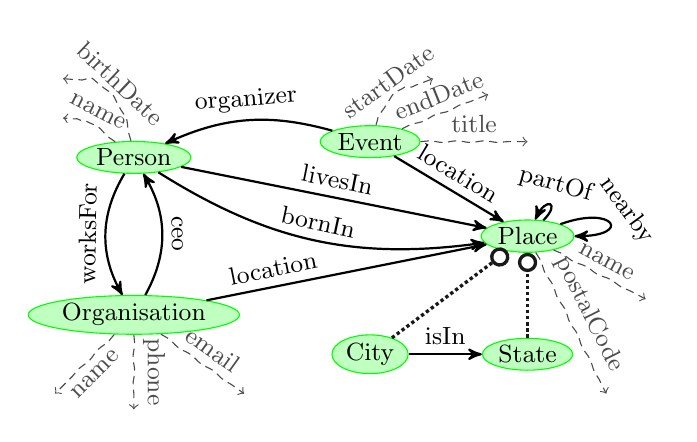
\begin{tikzpicture}
	\node[class] (pe) at (0,0)  {Person};
	\node[class] (co) at (0,-2) {Organisation};
	\node[class] (ev) at (3,0.2) {Event};
	\node[class] (pl) at (5,-1) {Place};
	\node[class] (ci) at (3,-2.5) {City};
	\node[class] (st) at (5,-2.5) {State};
	
		
	\path[hasaC,->] (pe) edge [bend left= -30] 
	node [midway, above, sloped] {worksFor} (co) ;
	\path[hasaC,->] (co) edge [bend left= -30] 
	node [midway, above, sloped] {ceo} (pe) ;
	
	\path[hasaC,->] (co) edge [] 
	node [near start, above, sloped] {location} (pl) ;
	
	\path[hasaC,->] (pe) edge [bend left = -20] 
	node [midway, above, sloped] {bornIn} (pl) ;
	\path[hasaC,->] (pe) edge [bend left = 0] 
	node [midway, above, sloped] {livesIn} (pl) ;
	
	\path[hasaC,->] (ev) edge [bend left = -20] 
	node [midway, above, sloped] {organizer} (pe) ;
	\path[hasaC,->] (ev) edge [bend left = 0] 
	node [midway, above, sloped] {location} (pl) ;
	
	
	\path[hasaC,->] (pl) edge [out=20,in=0,looseness=8] 
	node [midway, above, sloped] {nearby} (pl) ;
	\path[hasaC,->] (pl) edge [out=45,in=65,looseness=8] 
	node [midway, above, sloped] {partOf} (pl) ;
	
	\path[hasaC,->] (ci) edge  []
	node [midway, above, sloped] {isIn} (st) ;
	
	\path[isa,->] (ci) -- node [] {} (pl) ;
	\path[isa,->] (st) -- node [] {} (pl) ;
	

	\path[draw,hasaA,->] (pe) edge [decorate,out=140,in=0] 
	node [midway, above, sloped] {name} (-0.9,0.5);
	\path[draw,hasaA,->] (pe) edge [decorate,out=100,in=0] 
	node [midway, above, sloped] {birthDate} (-0.9,1);	
	
	\path[draw,hasaA,->] (co) edge [decorate,bend left = 0] 
	node [midway, below, sloped] {name} (-1,-3);
	\path[draw,hasaA,->] (co) edge [decorate,bend left = 0] 
	node [midway, above, sloped] {phone} (0,-3.2);
	\path[draw,hasaA,->] (co) edge [decorate,bend left = 0] 
	node [midway, above, sloped] {email} (1.4,-3);
	
	\path[draw,hasaA,->] (ev) edge [decorate,out=70,in=200] 
	node [midway, above, sloped] {startDate} (3.8,1);
	\path[draw,hasaA,->] (ev) edge [decorate,bend left = 0] 
	node [midway, above, sloped] {endDate} (4.5,0.8);
	\path[draw,hasaA,->] (ev) edge [decorate,bend left = 0] 
	node [midway, above, sloped] {title} (5,0.2);
	
	\path[draw,hasaA,->] (pl) edge [decorate,bend left = 0] 
	node [midway, above, sloped] {name} (6.5,-1.8);
	\path[draw,hasaA,->] (pl) edge [decorate,bend left = 0] 
	node [midway, above, sloped] {postalCode} (6,-3);	
	

\end{tikzpicture}
\caption{Example of ontology
(`\tikz{ \node[class, inner sep = 2] () at (0,0)  {};}' are Classes, `\tikz{ \path[hasaC,->] 
(0,1) -- (3ex,1);}' means ``has an object property'', 
`\tikz{ \path[hasaA,decoration={post length=0}] (0,0) edge[decorate] (3ex,0);}' 
means ``has a data property'' and 
`\tikz{ \path[isa,->] (0,1) -- (3ex,1);}' means ``is a'' ). Example by
\citeasnoun{Taheriyan2013}.
}
\label{FIG:onto}
\vspace{-3mm}
\end{figure}

In our work we consider that an ontology $\mathcal{O}$ includes basic elements such 
as classes (which represent concepts), literal values, individuals (members of classes) and properties~\cite{Spanos:semweb}.
Properties are classified into \emph{object properties}, which relate two 
individuals, 
and \emph{datatype properties}, which relate individuals to literal values.
Fig.~\ref{FIG:onto} gives an example of an ontology. 
Here, an individual of the class ``Organisation'' can be related to an individual of the class ``Person'' via object properties ``ceo'' or ``worksFor'', and it can have a data property ``name''. 
We also consider a special ``subclass'' (or ``is-a'') type of object properties.
For 
example, ``Cities'' and ``States'' are both ``Places''. 
A subclass inherits all the properties of the parent class.

A \emph{semantic model} $m$ is a directed graph with two types of nodes: 
\emph{class nodes} and \emph{data nodes}. 
We denote them as $\mathcal{C}_m$ and $\mathcal{D}_m$ respectively.
$ \mathcal{C}_m$ corresponds to classes in the ontology 
whereas $\mathcal{D}_m$ corresponds to data 
properties. 
Edges in the semantic model correspond to properties in the ontology, as 
shown in Fig.~\ref{FIG:sem} (notice the same edges appear in Fig.~\ref{FIG:onto}).
The semantic model may have several instances of the same ontology class, that is why class nodes are enumerated.

\begin{figure}[ht]
\centering
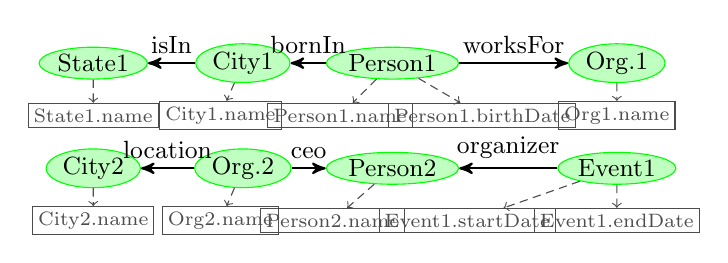
\begin{tikzpicture}[scale=0.95]
\begin{scope}
	\node[class] (pe) at (3,0)  {\small Person1};
	\node[class] (co) at (6,0) {\small Org.1};
	\node[class] (ci) at (1,0) {\small City1};
	\node[class] (st) at (-1,0) {\small State1};
	
	\node[data] (pen) at (2.3,-0.7) {\scriptsize Person1.name};
	\node[data] (peb) at (4.2,-0.7) {\scriptsize Person1.birthDate};
	\node[data] (cin) at (0.7,-0.7) {\scriptsize City1.name};
	\node[data] (stn) at (-1,-0.7) {\scriptsize State1.name};
	\node[data] (con) at (6,-0.7) {\scriptsize Org1.name};
	
		
	\path[hasaC,->] (pe) edge [bend left= 0] 
	node [midway, above, sloped] {worksFor} (co) ;
	
	
	\path[hasaC,->] (pe) edge [bend left = 0] 
	node [midway, above, sloped] {bornIn} (ci) ;
	
	
	\path[hasaC,->] (ci) edge  []
	node [midway, above, sloped] {isIn} (st) ;

	

	\path[draw,hasaA,->] (pe) -- (pen);
	\path[draw,hasaA,->] (pe) -- (peb);	
	
	\path[draw,hasaA,->] (co) -- (con);
	
	\path[draw,hasaA,->] (ci) -- (cin);
	
	\path[draw,hasaA,->] (st) -- (stn);
\end{scope}
\begin{scope}[yshift=-40]
	\node[class] (pl) at (-1,0)  {\small City2};
	\node[class] (pe) at (3,0)  {\small Person2};
	\node[class] (co) at (1,0) {\small Org.2};
	\node[class] (ev) at (6,0) {\small Event1};
	
	\node[data] (pen) at (2.2,-0.7) {\scriptsize Person2.name};
	\node[data] (evs) at (4,-0.7) {\scriptsize Event1.startDate};
	\node[data] (eve) at (6,-0.7) {\scriptsize Event1.endDate};
	\node[data] (con) at (0.7,-0.7) {\scriptsize Org2.name};
	\node[data] (pln) at (-1,-0.7) {\scriptsize City2.name};
	
		
	\path[hasaC,->] (co) edge [bend left= 0] 
	node [midway, above, sloped] {ceo} (pe) ;
	
	
	\path[hasaC,->] (ev) edge [bend left = 0] 
	node [midway, above, sloped] {organizer} (pe) ;
	
	\path[hasaC,->] (co) edge [bend left = 0] 
	node [midway, above, sloped] {location} (pl) ;



	\path[draw,hasaA,->] (pl) -- (pln);	

	\path[draw,hasaA,->] (pe) -- (pen);
	
	\path[draw,hasaA,->] (co) -- (con);
	
	\path[draw,hasaA,->] (ev) -- (evs);
	\path[draw,hasaA,->] (ev) -- (eve);
	
\end{scope}
\end{tikzpicture}
\caption{Examples of two semantic models (`\tikz{ \node[class, inner sep = 2] () at (0,0)  
{};}' are class nodes, and `\tikz{ \node[data] () at (0,0)  {};}' are data 
nodes).}
\label{FIG:sem}
\vspace{-3mm}
\end{figure}

In our setting we work with relational sources.
Hence, a \emph{data source} $s$ is a $n$-ary relation with a set of attributes 
$\mathcal{A}_s = (a_1,...,a_n)$.
We want to map them to the target ontology $\mathcal{O}$.

Following the traditional data integration framework~\cite{doan2012principles}, we decompose the problem into two parts: schema matching and schema mapping.
Schema matching, which we refer to as \emph{semantic labeling}, finds 
correspondences between attributes from data sources and data nodes of the 
target ontology.
In the schema mapping part we want to generate the semantic models of data sources by identifying the connecting paths for the matched data nodes.

An \emph{attribute mapping} function $\phi : \mathcal{A}_s \mapsto 
\mathcal{D}_m$ is a function which maps the attributes of the source $s$ into the nodes of the semantic model $m$. 
It can be a partial mapping, meaning that only some of the attributes
are connected to the nodes of $m$.
The attribute mapping function addresses the first part of the problem (i.e. the semantic labeling).

We define a \emph{source description} as a triple $\delta = (s, m, \phi)$ where $s$ is a source, $m$ is a semantic model, and $\phi$ is an attribute mapping.
Our problem can hence be stated as follows. We have an ontology 
$\mathcal{O}$ and a set of source descriptions $S_T = \{(s_1, m_1, \phi_1),..., 
(s_l, m_l, \phi_l)\}$.
Given a new source $s^\star$, we want to build a semantic model $m^\star$ and an attribute mapping function $\phi^\star$ such that 
$\delta^\star = (s^\star,m^\star,\phi^\star)$ is an \emph{appropriate} source description. 
We use the term ``appropriate'' since there might be many such triples which are well-formed source descriptions, 
but only one or a few will capture the intended meaning of the source. 
Our goal is to automatically build $\delta^\star$ such that it maximizes the \emph{precision} and \emph{recall} between the semantic model 
$m^\star$ and the semantic model $m^\dag$ that the user considers correct. 
%\npr{definitions for precision and recall}


\section{ML for Training on Source Descriptions \label{SEC:ML}}


\subsection{Semantic Labeling}
The semantic types $\mathcal{L_O} = \{l_1, l_2, ..., l_p\}$ of an ontology 
correspond to all pairs $(c,d)$, where $c$ is a Class in $\mathcal{O}$, and $d$ 
is a data property of that class (including inherited properties). 
For example, from the ontology in Fig. \ref{FIG:onto}, we would get
(City,name) and (State,name).

The first step to model the semantics of a new source $s^\star$ is to recognize the semantic types present in the source. 
We call this step \emph{semantic labeling}, which assigns a confidence value to a match of an attribute from $s^\star$ to a type $l \in 
\mathcal{L_O}$.
Typically semantic labeling techniques encounter several problems.
Firstly, there can be naming conflicts~\cite{Pinkel:rodi}, including those 
cases where users represent the same data in different ways.
Secondly, semantically different attributes might have syntactically similar 
content, for example, startDate versus endDate for the Event class.
Thirdly, there may be a considerable number of attributes which do not have any 
corresponding property in the ontology, either by accident or deliberately.
%\ddg{CHECK!}

We formulate the problem of semantic labeling as a multi-class classification
problem.
The known source descriptions $S_T$ provide us the training sample.
We compute a feature vector for each attribute in a data source and associate 
the known semantic type with the corresponding feature vector.
The feature vector includes, among others, characteristics
such as a number 
of whitespaces and other special characters, statistics of 
values in the column. 
A full list can be found in Appendix \ref{Ann:SemLab}.
%\npr{If I remove entropy descr, we are perfectly within page limit}
%\ignore{
One of the important features characterising information content of an attribute is Shannon's entropy.
% of the attribute's concatenated rows
Shannon's entropy 
%(or information entropy~\cite{Manning:Introduction})
 of a string $X$ is defined as
$H(X) = -\sum_{i}{p_i \log_{2}p_i},$ where $p_i$ is the probability of a character, whose index in character vocabulary is $i$, to appear in $X$, and the summation ranges over all
characters in the vocabulary.
%of all possible characters
To evaluate $p_i$ in Shannon's entropy, we evaluate normalized character frequency distribution \emph{chardist} of an attribute, as character counts in concatenated rows of the attribute, normalized by the total length of the concatenated rows.
The vocabulary of all characters consists of 100 printable characters (including $\backslash$n).
Finally, we add the 100-dimensional vector of $p_i$ to the attribute feature vector.
%}
We also compute a set of features based on similarity metrics inspired by state-of-the-art works by ~\citeasnoun{Pham:semantic} or~\citeasnoun{Ritze:matching}.
Among others, we compute mean cosine similarity for character distributions of attribute values and string similarity metrics for attribute names.
%To extract features from attribute names, we compute string similarity metrics: minimum edit distance, two WordNet based similarity measures such as JCN~\cite{Jiang:Semantic} and LIN ~\cite{Lin:Information}, and $k$-nearest neighbors using Needle-Wunsch distance~\cite{Needleman:General}.
%The minimum edit distance between two strings $s_1$ and $s_2$ is the minimum number of edit operations, such as insertion, deletion, substitution, which are required to transform one string into another~\cite{Manning:Introduction}.
%We compute the similarity between attribute name and all class instances in the training data.
%The number of thus extracted features depends on the number of semantic labels in the training data.
We train a random forest on the obtained sample. 

In this way, we learn the mapping $\psi : \mathcal{A}_s \times \mathcal{L_O} 
\mapsto [0, 1]$,
where $\psi(a_i,l_j)$ indicates the confidence that the attribute $a_i$ is 
mapped to the semantic type $l_j$.

Note that we keep all the matches, regardless of the confidence of the match. 
This is an important difference between our system and other approaches 
\cite{taheriyan2016learning} that 
remove some of the matches based on heuristics in order to simplify the task of 
finding the semantic model. 
%\ddg{is this last paragraph true?} \npr{yes}

%\ddg{IMPORTANT: Do we keep  all of them, or only the top $k$ with most 
%confidence? If so, 
%what is $k$?}
%\npr{We keep all, that is the crucial difference from Karma which does some 
%voodoo heuristic filtering}


\subsection{Alignment Graph}

To provide an integrated view over the known source descriptions $S_T$, we 
need to align their semantic models as well as all considered semantic 
types. 
This is achieved by constructing an \emph{alignment graph}. 

The alignment graph is a directed weighted graph $\mathcal{G_O} = 
(\mathcal{V_O},\mathcal{E_O})$ built on top 
of the known semantic models and expanded using the semantic types 
$\mathcal{L_O}$ and the ontology $\mathcal{O}$. 
Similar to a semantic 
model, $\mathcal{G_O}$ contains both class and data nodes.
The links correspond 
to properties in  $\mathcal{O}$ and are weighted \cite{taheriyan2016learning}.

The algorithm we use for the construction of the alignment graph 
$\mathcal{G_O}$ was given by~\citeasnoun{taheriyan2016learning}.
Briefly, it has three parts:
%\begin{enumerate}
$(i)$ %\item 
Adding the known semantic models
$(ii)$ %\item 
Adding the semantic types learned for the target source
%\item 
$(iii)$ Expanding the graph using the domain ontology.
%\end{enumerate}

Note how the alignment graph contains data nodes that correspond to semantic types. 
For instance, it could contain two nodes $City.name$ and $State.name$ rather than just one node $name$ connected to two 
nodes $City$ and $State$. 
We say these nodes are \emph{induced} into the 
alignment graph by the semantic types.
We note them $\mathcal{D_{G_O}}$ and call them the \emph{data nodes} of the alignment graph.
Class nodes are noted $\mathcal{C_{G_O}}$.

The graph is weighted by a function $w_\mathcal{O} : \mathcal{E_O} \mapsto 
\mathbb{R}$ such that edges which are present in
the known semantic models have lower weights than those 
which are inferred from the ontology.
In the next section we will see that this makes edges from semantic models 
more attractive. 
\citeasnoun{taheriyan2016learning} provide details on the weighting function.
%\ddg{How exactly are they weighted?}

An example alignment graph is illustrated in Fig.~\ref{FIG:ali}. 
%Bigger examples can be found in \cite{Taheriyan2013}. 
Black links correspond to the links which are supported by the known semantic models. 
Blue and orange links are inferred from the ontology $\mathcal{O}$ (the orange 
ones correspond to the ones added to connect Classes of the ontology that never 
appeared in the semantic models).
% and can be assigned the 
%maximum weight $w_max$ \ddg{where does this weight come from?}


\begin{figure}[ht]
\centering
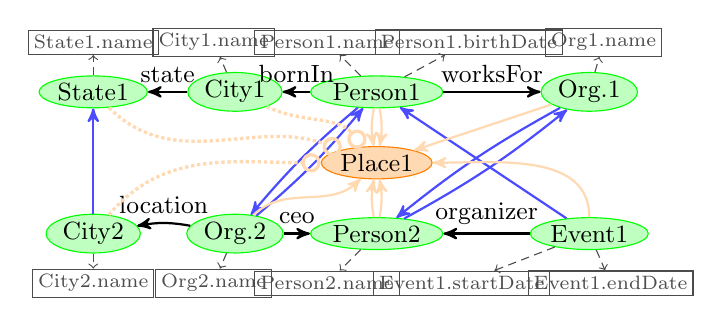
\begin{tikzpicture}[scale=0.9]

	\node[class] (pe1) at (3,0)  {\small Person1};
	\node[class] (co1) at (6,0) {\small Org.1};
	\node[class] (ci1) at (1,0) {\small City1};
	\node[class] (st1) at (-1,0) {\small State1};
	
	\node[data] (pen) at (2.3,0.7) {\scriptsize Person1.name};
	\node[data] (peb) at (4.3,0.7) {\scriptsize Person1.birthDate};
	\node[data] (cin) at (0.7,0.7) {\scriptsize City1.name};
	\node[data] (stn) at (-1,0.7) {\scriptsize State1.name};
	\node[data] (con) at (6.2,0.7) {\scriptsize Org1.name};
	
		
	\path[hasaC,->] (pe1) edge [bend left= 0] 
	node [midway, above, sloped] {worksFor} (co1) ;
	
	
	\path[hasaC,->] (pe1) edge [bend left = 0] 
	node [midway, above, sloped] {bornIn} (ci1) ;
	
	
	\path[hasaC,->] (ci1) edge  []
	node [midway, above, sloped] {state} (st1) ;

	

	\path[draw,hasaA,->] (pe1) -- (pen);
	\path[draw,hasaA,->] (pe1) -- (peb);	
	
	\path[draw,hasaA,->] (co1) -- (con);
	
	\path[draw,hasaA,->] (ci1) -- (cin);
	
	\path[draw,hasaA,->] (st1) -- (stn);


% % % CC2
\def\ysh{-2};

	\node[class] (pl2) at (-1,0+\ysh)  {\small City2};
	\node[class] (pe2) at (3,0+\ysh)  {\small Person2};
	\node[class] (co2) at (1,0+\ysh) {\small Org.2};
	\node[class] (ev2) at (6,0+\ysh) {\small Event1};
	
	\node[data] (pen) at (2.3,-0.7+\ysh) {\scriptsize Person2.name};
	\node[data] (evs) at (4.2,-0.7+\ysh) {\scriptsize Event1.startDate};
	\node[data] (eve) at (6.3,-0.7+\ysh) {\scriptsize Event1.endDate};
	\node[data] (con) at (0.7,-0.7+\ysh) {\scriptsize Org2.name};
	\node[data] (pln) at (-1,-0.7+\ysh) {\scriptsize City2.name};
	
		
	\path[hasaC,->] (co2) edge [bend left= 0] 
	node [midway, above, sloped] {ceo} (pe2) ;
	
	
	\path[hasaC,->] (ev2) edge [bend left = 0] 
	node [midway, above, sloped] {organizer} (pe2) ;
	
	\path[hasaC,->] (co2) edge [bend left = -10] 
	node [midway, above, sloped] {location} (pl2) ;



	\path[draw,hasaA,->] (pl2) -- (pln);	

	\path[draw,hasaA,->] (pe2) -- (pen);
	
	\path[draw,hasaA,->] (co2) -- (con);
	
	\path[draw,hasaA,->] (ev2) -- (evs);
	\path[draw,hasaA,->] (ev2) -- (eve);
	

% % % Ontology

	\path[draw,hasaC,->,blue!70] (co2)  edge [bend left = -5] (pe1);
	\path[draw,hasaC,->,blue!70] (pe1)  edge [bend left = -5] (co2);
	
	\path[draw,hasaC,->,blue!70] (co1)  edge [bend left = -5] (pe2);
	\path[draw,hasaC,->,blue!70] (pe2)  edge [bend left = -5] (co1);

	\path[draw,hasaC,->,blue!70] (pl2) -- (st1);
	
	\path[draw,hasaC,->,blue!70] (ev2) -- (pe1);
	
	
	\node[class,orange,fill=orange!30!white,text=black] (PL) at (3,\ysh/2)  
	{\small 
	Place1};
	
	\path[draw,hasaC,->,orange!30!white] (pe1) edge[bend left=10] (PL);
	\path[draw,hasaC,->,orange!30!white] (pe1) edge[bend left=-10] (PL);
	
	\path[draw,hasaC,->,orange!30!white] (pe2) edge[bend left=10] (PL);
	\path[draw,hasaC,->,orange!30!white] (pe2) edge[bend left=-10] (PL);
	
	\path[draw,hasaC,->,orange!30!white] (co1) edge[bend left=0] (PL);
	\path[draw,hasaC,->,orange!30!white] (co2) edge[out=45,in=225] (PL);

	\path[draw,hasaC,->,orange!30!white] (ev2) edge[out=90,in=0] (PL);
	
	\path[draw,isa,->,orange!30!white] (ci1) edge[out=-25,in=130] (PL);
	\path[draw,isa,->,orange!30!white] (pl2) edge[out=50,in=180] (PL);
	\path[draw,isa,->,orange!30!white] (st1) edge[out=-45,in=160] (PL);

\end{tikzpicture}
\caption{Example of alignment graph (`\tikz{ \node[class, inner sep = 2] () at (0,0)  
{};}' `\tikz{ \node[class,orange,fill=orange!30!white,text=black, inner sep = 2] () at 
(0,0)  
{};}' are class nodes, and `\tikz{ \node[data] () at (0,0)  {};}' are data 
nodes). We omit weights for clarity.}
\label{FIG:ali}
\vspace{-3mm}
\end{figure}


\subsection{Frequent Graph Pattern Mining \label{SSEC:pattern-mining}}

Certain patterns of connections can be prevalent in the domain.
For example, in Fig.~\ref{FIG:sem} both semantic models have class nodes ``City'', ``Organization'' and ``Person''.
According to the ontology in Fig.~\ref{FIG:onto} there are multiple ways to connect these nodes.
However, if we know that the ``Person'' works for the ``Organization'', then based on the known semantic models (Fig.~\ref{FIG:sem}), ``City'' is more likely to be the birth place of the ``Person'' rather than the location of the ``Organization''.
To increase the coherence of the generated semantic models, we would like to discover such patterns of connections.

%As an extension to the problem, we consider using pattern mining techniques in order to identify patterns in the training set of semantic model that repeat themselves often. 
%The hope is that with such information we can encourage the semantic model $m^\star$ for the new source to use groups of edges that                                       appeared often together in training semantic models.

%\npr{reformulate for typed directed multigraphs and example based on Fig3}
In our context, patterns are typed directed graphs.
We mine these patterns from the set of semantic models in the training set $S_T$.
This is known as Transactional Frequent Graph Pattern Mining, which
includes the subgraph isomorphism problem, known to be NP-complete.
The frequency of a pattern is the number of semantic models 
which contain
at least one subgraph isomorphic to the pattern.
The \emph{support} of the pattern is calculated as its 
frequency relative to the number of semantic models.
This is an anti-monotonous measure, meaning that bigger 
patterns will have lower supports than their subgraphs.
% \ddg{Define support}
We solve the pattern mining task with the tool DIMSpan \cite{petermann2017dimspan} which adapts gSpan~\cite{yan2002gspan} pruning techniques to the typed graphs and uses Apache Flink for scalability.  
We obtain patterns of size up to 6 in under 4 minutes for the biggest instances 
in our evaluation framework.
Hence, this pattern mining procedure is a highly 
scalable approach compared to the technique based on SPARQL queries 
from~\cite{Taheriyan:Leveraging}.
%\npr{Elaborate more, karma's approach for pattern mining took 1 hour, maybe 
%cite my work on how databases perform for graph pattern matching. Should it be 
%better in related work?}

%Let $G = (V_G,E_G,\lambda_G)$ and $P = (V_P,E_P, \lambda_P)$ be two graphs 
%where $\lambda_G$ (resp. $\lambda_P$) is a \emph{labeling function} that maps 
%nodes/edges of $G$ (resp. $P$) into a set of labels (e.g. natural numbers).
%An \emph{embedding} of $P$ into $G$ is an injective function $f : V_G \mapsto 
%V_P$ such that for all $x,y \in V_P$:
%\begin{enumerate}
%	\item $\{x,y\} \in E_P \implies \{f(x),f{y}\} \in E_G$.
%	\item $\lambda_P(x) = \lambda_G(f(x))$
%	\item $\lambda_P(\{x,y\}) = \lambda_G(\{f(x),f(y)\})$
%\end{enumerate} 
%That is, if an edge exists in $P$, it must also exist in $G$ (but not 
%vice-versa); and the labelling functions of both graphs must match after 
%applying the embedding function.

%Our goal is to take a set of graphs (the semantic models from the training set 
%$S_T$) and find patterns that appear often across that set of graphs. 
%This is 
%known as the Frequent Graph Pattern Mining, which contains the subgraph 
%isomorphism, known to be NP-complete.  
%We solve this task with the tool DIMSpan \cite{petermann2017dimspan} which adapts gSpan~\cite{yan2002gspan} pruning techniques to the typed graphs and uses Apache Flink for scalability. 
%\ddg{CHECK! How do they solve an NP-complete problem??}
%\npr{Im not sure what to say here: there is just no guarantee how long it will take for the whole thing to run, except there is a threshold on how frequent they have to be; they use gSpan procedure to prune patterns and a variant of Ulmans algorithm for graph pattern matching}
% 
%This tool provides us with a list of patterns that are frequent, as well as 
%their support. 
%The \emph{support} of a pattern is an anti-monotonous measure of frequency. 
%Thus, the higher the support, the more often the pattern appears. 
%This typically means that big patterns have low support.
 

\section{Steiner Tree Formulation \label{SEC:STP}}

Given a graph $G =
(V, E)$ and a subset of its nodes $T \subseteq V$, a 
Steiner Tree $G_s = (V_s, E_s )$ is a tree (connected acyclic graph) such that 
$T \subseteq V_s \subseteq 
V$ and $E_s \subseteq E$. 
In other words, $G_s$ spans all the nodes in $T$ and 
may include additional nodes from $V$, in particular to ensure the 
connectedness of the constructed tree. 
The Steiner Tree Problem 
(STP) is stated as follows: given $G$ and a weight function $w_f : E 
\mapsto \mathbb{R}$, find the Steiner Tree that minimizes the sum of the 
weights of the edges in $E_s$ given by $w_f$. This was proven to be NP-hard 
by \citeasnoun{Karp1972}.

To formulate the \relonto{} schema mapping problem as a STP for a new source 
$s^\star$, we construct the 
\emph{integration graph} $~\mathcal{I}_\mathcal{O}^{s^\star} = 
(\mathcal{V}_\mathcal{O}^{s^\star},\mathcal{E}_\mathcal{O}^{s^\star})$, where  
$\mathcal{V}_\mathcal{O}^{s^\star} = \mathcal{V_O} \cup 
\mathcal{A}_{s^\star}$.

The set of edges $\mathcal{E}_\mathcal{O}^{s^\star}$ is constructed by using 
all the edges in the alignment 
graph, and edges connecting each attribute of $s^\star$ to the nodes in the 
alignment graph \emph{induced} by the semantic types (i.e. the set of nodes in 
$\mathcal{D_{G_O}}$). We call this last set 
of edges $\mathcal{M}_\mathcal{O}^{s^\star}$ (for ``matches''). Thus, 
$\mathcal{E}_\mathcal{O}^{s^\star} = 
\mathcal{E_O} \cup \mathcal{M}_\mathcal{O}^{s^\star}$.

We associate a weighting function  $w_\mathcal{I} : E \mapsto \mathbb{R}^+$ to 
the integration graph. 
For an edge $e \in \mathcal{E_O}$, $w_\mathcal{I}(e) = 
w_\mathcal{O}(e)$. For an edge $e 
\in \mathcal{M}_\mathcal{O}^{s^\star}$ connecting attribute $a_i$ to the node 
$l_j$ induced by the semantic model, $w_\mathcal{I}(e) = - 
ln(\psi(a_i,l_j))$, making unlikely matches have a higher weight. %\ddg{CHECK!}
An example of an integration graph can be found in Fig. \ref{FIG:inte}.




\begin{figure}[ht]
\centering
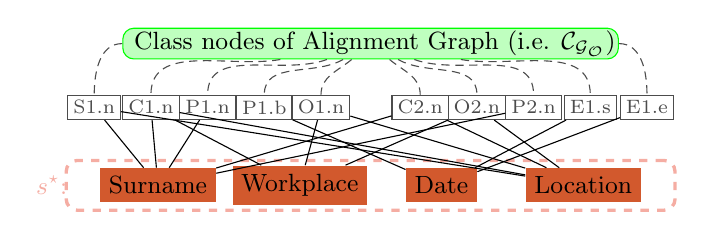
\begin{tikzpicture}[scale=0.9]
	\node[class, rectangle, rounded corners] (CLASS) at (0,0) { \small{ 
	Class nodes of Alignment Graph (i.e. $\mathcal{C_{G_O}}$)}};
	
	\node[data] (stn1) at (-3.9,-0.9) {\scriptsize S1.n};
	\node[data] (cin1) at (-3.1,-0.9) {\scriptsize C1.n};
	\node[data] (pen1) at (-2.3,-0.9) {\scriptsize P1.n};
	\node[data] (peb1) at (-1.5,-0.9) {\scriptsize P1.b};
	\node[data] (con1) at (-0.7,-0.9) {\scriptsize O1.n};
	
	\path[draw,hasaA] (CLASS) edge[out=180,in=90] (stn1);
	\path[draw,hasaA] (CLASS) edge[out=190,in=90] (cin1);	
	\path[draw,hasaA] (CLASS) edge[out=200,in=90] (pen1);
	\path[draw,hasaA] (CLASS) edge[out=210,in=90] (peb1);	
	\path[draw,hasaA] (CLASS) edge[out=220,in=90] (con1);


% % % CC2
\def\ysh{0.1};
	
	\node[data] (cin2) at (0.7,-1+\ysh) {\scriptsize C2.n};
	\node[data] (con2) at (1.5,-1+\ysh) {\scriptsize O2.n};
	\node[data] (pen2) at (2.3,-1+\ysh) {\scriptsize P2.n};
	\node[data] (evs2) at (3.1,-1+\ysh) {\scriptsize E1.s};
	\node[data] (eve2) at (3.9,-1+\ysh) {\scriptsize E1.e};
	
	\path[draw,hasaA] (CLASS) edge[out=320,in=90] (cin2);	
	\path[draw,hasaA] (CLASS) edge[out=330,in=90] (con2);
	\path[draw,hasaA] (CLASS) edge[out=340,in=90] (pen2);
	\path[draw,hasaA] (CLASS) edge[out=350,in=90] (evs2);
	\path[draw,hasaA] (CLASS) edge[out=360,in=90] (eve2);
	
\node[rectangle, rounded corners,very thick,draw, dashed, 
brown!40!red!40!white,minimum 
height=18, minimum 
width=220] 
(source) at 
(0,-2) 
{};
\node[brown!40!red!40!white] 
(source) at 
(-4.5,-2) 
{$s^\star$:};
	\node[att] (a1) at (-3,-2) {\small Surname};
	\node[att] (a2) at (-1,-2) {\small Workplace};
	\node[att] (a3) at (1,-2) {\small Date};
	\node[att] (a4) at (3,-2) {\small Location};

	\path[draw] (a1) -- (stn1);
	\path[draw] (a1) -- (cin1);
	\path[draw] (a1) -- (pen1);
	\path[draw] (a1) -- (cin2);
	\path[draw] (a1) -- (pen2);
	
	\path[draw] (a2) -- (cin1);
	\path[draw] (a2) -- (con1);
	\path[draw] (a2) -- (con2);

	\path[draw] (a3) -- (peb1);
	\path[draw] (a3) -- (evs2);
	\path[draw] (a3) -- (eve2);

	\path[draw] (a4) -- (stn1);
	\path[draw] (a4) -- (cin1);
	\path[draw] (a4) -- (con1);
	\path[draw] (a4) -- (cin2);
	\path[draw] (a4) -- (con2);
\end{tikzpicture}
\caption{Example of integration graph. (`\tikz{ \node[att] () at (0,0)  
{};}' are attribute nodes). We omit weights and only show the most likely 
matches for clarity. Data node
are the same as in Fig \ref{FIG:ali}.}
\label{FIG:inte}
\vspace{-3mm}
\end{figure}

Note that, although the alignment graph is directed, we disregard the
direction of edges for the STP model.
We disambiguate the direction and semantics of edges via their
weights.
We can further improve this step by using patterns.
%\npr{this was not completely correct}
%the semantic models are 
%not necessarily rooted graphs (e.g. Fig. \ref{FIG:sem}), therefore the 
%direction of the edges is ignored for the STP model (and are all treated as 
%undirected edges). 

The goal is to build a subgraph $T^\star= (V^\star, E^\star)$ of
$\mathcal{I}_\mathcal{O}^{s^\star}$ for the new source $s^\star$. The solution 
$T^\star$ will 
be used to build the source description $\delta^\star$. 
In particular, $(\mathcal{V_O} \cap V^\star,\mathcal{E_O} \cap E^\star)$ 
corresponds to the semantic model, and 
$(\mathcal{A}_{s^\star},\mathcal{M}_\mathcal{O}^{s^\star} \cap E^\star)$ 
corresponds to 
the attribute mapping function.

The solution $T^\star$ must satisfy the following constraints:
%\begin{enumerate}
	$(i)$ %\item 
	$T^\star$ must be a subgraph of $\mathcal{I}_\mathcal{O}^{s^\star}$,
	$(ii)$ %\item 
	$T^\star$ must be a tree,
	$(iii)$ %\item 
	$\forall a \in \mathcal{A}_{s^\star}, a\in V^\star$,
	$(iv)$ %\item 
	$\forall a \in \mathcal{A}_{s^\star}, degree(a) = 1$,
	%\item $\forall n \in \mathcal{D_{G_O}}, degree(a) \in 
	%\{0,2\}$
	$(v)$ %\item 
	$\forall n \in \mathcal{D_{G_O}} \cap V^\star, degree(n) = 2$,
	$(vi)$ 
	$V^\star \cap \mathcal{C_{G_O}} \neq \emptyset$.
%\end{enumerate}

It is therefore natural to model this problem as a STP with side constraints.
%, since the two first requirements imply that $T^\star$ is
%a Steiner Tree of the integration graph. 
By designing the weighting function $w_\mathcal{I}$ through 
ML techniques, as shown in Section \ref{SEC:ML}, 
our expectation is that the minimum cost Steiner Tree is a valid and coherent semantic model for the new source.


\subsection{Using Patterns}

As explained in Subsection \ref{SSEC:pattern-mining}, we also use 
graph patterns in order to incentivise the solution tree 
$T^\star$ to contain subgraphs of the alignment graph that have been frequently 
seen in the training set.
To do this, we use the support of each of the obtained patterns as a prize. If 
the tree contains a pattern, then its weight is automatically reduced by the 
value of the support of that pattern. We will see in the next section how this 
information is integrated in the model.

\subsection{Unmatched Attributes}
It is common that the data sources to be integrated will have columns that 
simply cannot be matched to the ontology.
This can happen when a column of a source table contains some information that 
is uninteresting to the user, or because the ontology has not been properly 
designed. 
Examples of these situations can be found in domain specific data 
\cite{Pham:semantic} or HTML tables \cite{Ritze:matching}.
In current systems, these columns are removed in a pre-processing step as a manual effort.

For this reason, we add two artificial Class nodes to the integration graph:  
\emph{unknown} and \emph{root}. 
The latter will be connected to every other Class node in 
$\mathcal{V}_\mathcal{O}^{s^\star}$, including \emph{unknown}.
We also add a set $U = \{unk_1,...,unk_{|\mathcal{A}_{s^\star}|}\}$ of 
$|\mathcal{A}_{s^\star}|$ data 
nodes to the integration graph each connected to exactly one node in 
$\mathcal{A}_{s^\star}$ and to the \emph{unknown} Class node.  

If an attribute $a$ is matched to $unk_a$, then $unk_a$ will be linked to Class 
node \emph{unknown}. 
The rest of the attributes can then be matched normally 
and build  a semantic model as usual. 
To maintain connectedness of the 
Steiner tree, the \emph{unknown} node and one of the other selected Class nodes 
will 
both be connected to the \emph{root} node. 
Note that if all attributes find a 
match, then both the \emph{unknown} and \emph{root} nodes will not be selected in 
the Steiner tree and the normal behavior will take place.
The weights of the edges between these special nodes are
assigned the same way as for the rest of the edges.
%\ddg{Explain the weights of the edges introduced by the unknown nodes}




\section{Modeling in Constraint Programming \label{SEC:CP}}
\subsection{Definitions}

A Constraint Optimization Problem (COP) is a tuple $P=(\boldsymbol{v},C,o)$ 
where $\boldsymbol{v}$ is a 
set of \emph{variables}, $C$ is a set of $n$-ary 
\emph{constraints} over variables $\boldsymbol{v}$ and $o$ is an 
\emph{objective function} $o : \boldsymbol{v} \mapsto \mathbb{R}$ to be 
(w.l.o.g.) minimized. 
A valuation such that all variables in $\boldsymbol{v}$ map 
to exactly one value, and all the constraints in $C$ are satisfied by the 
valuation is a \emph{solution} to $P$. A solution $\theta$ is optimal if$\not 
\exists \theta', \theta'(\boldsymbol{v}) < \theta(\boldsymbol{v})$.

Constraint Programming (CP) allows the user to model a COP and give it 
to a solver that will find solutions while optimizing 
the objective function (and prove optimality).

Briefly, the way a CP solver works is by assigning a value to each variable of 
$\boldsymbol{v}$ in turn. 
\ignore{At each iteration it will check whether any 
constraint in $C$ is violated, in which case it will backtrack to change its 
last decision. \ignore{The choice of the order of the variables to be assigned, 
and the 
choice of the value to be assigned to each variable is called the \emph{search 
strategy}.}}
CP uses a combination of complete search and \emph{propagation}. The latter
removes inconsistent values 
from the domains of variables. That way, values that cannot appear in a 
solution, given the current set of decisions, are never tried by the search. 
\emph{Global constraints} are higher order constraints that enforce a 
complex 
constraint over a set of variables. They are implemented with 
specialized algorithms for performance.


\subsection{\relonto{} in Constraint Programming}
In order to model this problem we used the \minizinc{} language 
\cite{minizinc}, and the 
\chuffed{} solver \cite{chu2011improving} because it has a global constraint 
implemented for Steiner 
Tree Problems \cite{deuna2016steiner}. The model can be found in Appendix \ref{Ann:MZ}.

Because attributes must be connected to exactly one node of the alignment 
graph, and that node will be in $\mathcal{D_{G_O}} \cap V^\star$ 
then the part of the problem between attribute nodes and the alignment graph is 
actually a matching problem. Each attribute must match exactly to one node of 
$\mathcal{D_{G_O}}$. Note that not all nodes in $\mathcal{D_{G_O}}$ need to match 
to an attribute, as not all of them are part of $T^\star$.

Because there are global constraints in CP specialized in matching 
\cite{regin1994filtering}, we split the problem into two parts: the 
$\mathit{steiner}$ global constraint \cite{deuna2016steiner} will only deal with the part of the 
integration graph that corresponds to the alignment graph, and the 
$\mathit{alldifferent}$ global constraint will deal with the matching part of 
the problem.

We use the following variables to represent the tree $T^\star$: Boolean 
variables $c_n,\forall n \in 
\mathcal{V_O}$, $c_e, \forall e \in	\mathcal{E_O}$ and an array of variables 
$match$ indexed by the set of attributes of $s^\star$. The combination of these 
sets of variables define the value of $T^\star$: $c_n = \mathit{true}$ means 
that $n \in V^\star$, $c_e = \mathit{true}$ means that $e \in E^\star$ and 
$match[a] = d$ (for $a \in \mathcal{A}_{s^\star}$ and $d \in 
\mathcal{D_{G_O}}$) means that the edge $(a,d) \in 
\mathcal{M}_\mathcal{O}^{s^\star}$ is part of $T^\star$.

Additionally, for a given set of patterns $\mathcal{P}$ with a support function 
$w_\mathcal{P} : \mathcal{P} \mapsto \mathbb{R}$, we have a set of Boolean 
variables 
$c_p, \forall p \in \mathcal{P}$ that tell us whether a pattern $p$ appears in 
$T^\star$ or not.
The model is presented below.

\begin{flalign}
	& \text{Minimize~~} w_{STP} + w_{ADIFF} - w_{PAT}
	%\sum_{e \in \mathcal{E}_\mathcal{O}}c_e * 
	%w_\mathcal{I}(e) + \sum_{e \in \mathcal{M}_\mathcal{O}^{s^\star}} c_e * 
    %		w_\mathcal{I}(e)
	\label{EQ:obj}~~~\text{such that~~} && \\
	& \textit{steiner}(\{c_n| n \in \mathcal{V_O}\},\{c_e| e \in 
	\mathcal{E_O}\},\mathcal{G_O},w_\mathcal{O},w_\mathit{STP})  \label{EQ:stp} 
	&&\\
	&\forall d \in \mathcal{D_{G_O}}, degree(d) \leq 1 \label{EQ:deg1}&&\\
	&\forall d \in \mathcal{D_{G_O}}, c_d \Leftrightarrow degree(d) = 1 
	\label{EQ:deg2}&&\\
	&\forall a \in \mathcal{A}_{s^\star}, match[a] \in \{ d | (a,d)\in 
	\mathcal{M}_\mathcal{O}^{s^\star} \} \label{EQ:matchdom}&&\\
	& \textit{alldifferent}(match) \label{EQ:alld}&& \\
	& \forall a \in \mathcal{A}_{s^\star}, c_{match[a]} = \mathit{true} 
	\label{EQ:map}&&\\
	& w_{\mathit{ADIFF}} = \sum_{(a,d) \in \mathcal{M}_\mathcal{O}^{s^\star}} 
	w_\mathcal{I}(~(a,d)~) * \llbracket match[a] = d\rrbracket 
	\label{EQ:matchcost}  &&\\
	& \forall p \in \mathcal{P}, \big(\forall e\in edges(p), c_e = 
	\mathit{true} \big) \Leftrightarrow c_p \label{EQ:patt}&&\\
	& w_{PAT} = \sum_{p\in\mathcal{P}} w_\mathcal{P}(p)* c_p 
	\label{EQ:pcost} &&\\
	& c_{unknown} \Rightarrow \big( c_{root}  \land 
	c_{(unknown,root)} \big) \label{EQ:unk}
\vspace{-3mm}
\end{flalign}

Eq.~\ref{EQ:obj} is the objective function: we are minimizing the cost 
of $T^\star$ while collecting prizes for each pattern we use. 
Eq.~\ref{EQ:stp} enforces that the solution 
$T^\star$ is indeed a tree defined by the $c_n$ and $c_e$ variables,
subgraph of the alignment graph 
and of total weight $w_{STP}$. 
Eq.~\ref{EQ:deg1} and \ref{EQ:deg2} ensure 
that if a data node of the alignment graph is selected, then at most one edge 
reaches it (from the side of the alignment graph) and otherwise it is 
disconnected. 
\ignore{Eq. \ref{EQ:matchdom} ensures that the domain of each 
variable in 
the array $match$ corresponds to a subset of data nodes of the alignment graph 
for which there is an edge connecting to the attribute at hand. 
Eq.~\ref{EQ:alld} ensure that each attribute is mapped to exactly one data node of 
the alignment graph.}
Eq.~\ref{EQ:matchdom} and \ref{EQ:alld} ensure that 
there is exactly one data node matched to an attribute. 
Eq.~\ref{EQ:map} ensures that 
if a data node of the alignment graph has been mapped to some attribute, then 
that data node must be in the solution tree, and vice-versa. 
Eq.~\ref{EQ:matchcost} computes the cost $w_{ADIFF}$ of the matches.
Eq.~\ref{EQ:patt} indicates that a pattern is used if and only if all its edges are selected in the tree. 
Eq.~\ref{EQ:pcost} computes the prizes collected by using patterns.
Eq. \ref{EQ:unk} ensures that if the \emph{unknown} class node is used, then it 
is connected to \emph{root}.
Notice there is no further requirement for unmatched attributes, as the 
$unk_i$ data nodes behave like normal data nodes, and the connectedness 
requirement will make sure that \emph{root} is connected to the rest of the 
tree (i.e. the semantic model).

Note how this CP model is easy to adapt to more classic settings where no 
patterns are used (by dropping Eqs. \ref{EQ:patt} and \ref{EQ:pcost}), or 
without \emph{unknown} nodes (by dropping Eq. \ref{EQ:unk}).

We choose a search strategy that will first try to match attributes using the cheapest edges in $\mathcal{M}_\mathcal{O}^{s^\star}$. Then, it will try to use the cheapest unfixed edge $e\in\mathcal{E_O}$ that fills a pattern $p$ (i.e. $\forall e_p\in p, e_p \neq e, c_{e_p}$) such that $w_\mathcal{P}(p) > w_\mathcal{O}(e)$ or simply the cheapest edge if none fill a pattern.

\section{Results \label{SEC:Res}}

\subsection{Experimental Setup}

% datasets for evaluation
For the rest of the paper, we call our system \serene{} if no patterns are used in the model, and \serenepats{} otherwise.

We run experiments on two domains: museum and soccer (see Fig.~\ref{tab:data} for statistics).
The museum dataset~\cite{taheriyan2016learning} contains 29 sources which are mapped to the EDM domain ontology.
The soccer dataset~\cite{Pham:semantic} is much smaller with only 12 data sources, and its domain ontology is an extension of the schema.org ontology.

\begin{table}[ht]\small
  \centering
  \caption{Description of data sources.}\label{tab:data}
		\begin{tabular}{ccccc}
		\hline
		\multirow{2}{*}{\textbf{Domain}} & \# data & \# semantic & \# & \# unknown\\
		 & sources & labels & attributes & attributes\\
		\hline
		museum & 29 & 20 & 443 & 159  \\
		soccer & 12 & 18 & 138 & 42 \\
		\hline
		\end{tabular} 
\end{table}

%\begin{table*}[ht]
%  \centering
%  \caption{Description of data sources.}\label{tab:data}
%		\begin{tabular}{ccccccc} 
%		\hline
%		\multirow{2}{*}{\textbf{Domain}} & \# & \# semantic & \# & \# unknown & avg \# rows & avg \# attributes\\
%		 & sources & labels & attributes & attributes & per source & per source\\
%		\hline
%		museum & 29 & 20 & 443 & 159 & 6978.89 & 15.27 \\
%		soccer & 12 & 18 & 138 & 42 & 2120.16 & 11.5 \\
%		\hline
%		\end{tabular} 
%\end{table*}

% baseline for evaluation
We choose \karma{}~\cite{taheriyan2016learning} as our baseline.
This system also phrases the \relonto{} problem as STP and decomposes it further into two parts.
However, it uses heuristic algorithms both for the matching and for the STP 
parts.
It solves the problems sequentially, i.e., once it produces a set of candidate 
mappings for attributes into the ontology, it fixes this set and moves
onto the STP part.
Additionally, it does not consider unmatched attributes in the sources.
To ensure that \karma{} also handles such attributes, we change its semantic 
labeling model, SemanticTyper~\cite{Ramnandan:Assigning}, to ours and we add a 
special \emph{unknown} ontology which gives specification for \emph{root} and 
\emph{unknown} nodes of the alignment graph.
The first modification also ensures the fairness of evaluation since both 
\karma{} and \serene{} will have the same matches for attributes.

% performance metrics
The performance of these systems is estimated in terms of \emph{precision} and \emph{recall}.
Assuming $m^\star$ is the predicted semantic model and $m^\dag$ is the correct semantic model, then:
$$\mathit{prec} = \frac{|\mathit{rel}(m^\star)\cap 
\mathit{rel}(m^\dag)|}{|\mathit{rel}(m^\star)|}, 
\mathit{recall} = \frac{|\mathit{rel}(m^\star)\cap 
\mathit{rel}(m^\dag)|}{|\mathit{rel}(m^\dag)|}$$
where $rel(m)$ is the set of triples $(u,e,v)$ with $e$ being an edge from the vertex $u$ to the vertex $v$ in the semantic model $m$.
\ignore{Since we want to estimate the accuracy of both the matching and STP 
parts,
we also include triples for attributes and data nodes into the corresponding 
sets.}
Note that unmatched attributes as well as \emph{unknown} and \emph{root} nodes are not part of these sets.
We also perform a modification to the ground truth semantic models:
if the true semantic label of an attribute $a$ is not present in any of the 
previously mapped data sources, we substitute it with $unk_a$ and map it to the 
\emph{unknown} class node.
In such way we validate how well the systems can detect earlier unseen cases.

% semantic labeling models
To illustrate that our semantic labeling model is better suited for the
matching task, 
we compare it against the state-of-the-art model \emph{DSL}~\cite{Pham:semantic} which was shown to perform 
even better than SemanticTyper. 
%\npr{not sure whether I should explain how this model works}
We use \emph{mean reciprocal rank} (MRR) to evaluate semantic labeling models.
This measure is useful to estimate how highly the true semantic label is ranked among top $k$ suggestions.
It is calculated the following way:
$MRR = \frac{1}{n}\sum_{i=1}^{n}{\frac{1}{rank_i}},$
where $rank_i$ is the rank of the correct semantic label for the attribute $a_i$ among the top $k$ predictions.


% evaluation strategy
We perform an evaluation strategy outlined by~\cite{taheriyan2016learning}.
Let $M_j$ be the set of $j$ known semantic models.
For each data source $s_i$ in the domain we perform experiments $t-1$ times,
where $t$ is the total number of data sources in the domain and each experiment has a different number of known semantic models $M_1, M_2, \ldots, M_{t-1}$.
The case with $M_{t-1}$ known semantic models corresponds to leave-one-out validation strategy. 
For example, in the soccer domain for the source $s_1$ we run experiments 11 times using $M_1=\{m_2\}, M_2=\{m_2, m_3\}, \ldots, M_{11}=\{m_2, m_3, \ldots, m_{12}\}$
We repeat the procedure for other data sources in the domain and then average the results.
This procedure ensures that each source is at least once in the training as well as testing datasets.


% architecture
We have run all our experiments on a Dell server with 252 GB of memory, 2 CPUs 
with 4 cores each.
%\npr{check characteristics, AWS machine is bigger}
In all our experiments we use a timeout threshold of 15s for \chuffed{}, which 
runs on a single core (thus easy to deploy on any user's machine).

\subsection{Experimental Results}

To evaluate our new system \serene{}, we show that its semantic labeling model 
produces more accurate matches for attributes and that the CP formulation leads 
to better semantic models in terms of precision and recall.

\ignore{We have developed a new approach for semantic labeling which can 
efficiently handle the \emph{unknown} class.}
\ignore{We demonstrate its efficiency by comparing against the state-of-the-art 
approach DSL~\cite{Pham:semantic}. } %Repeat from above
Tab.~\ref{tab:semlab} provides evidence that our new semantic labeling model is better suited for the task when there are unmatched attributes in domains.
DSL uses heuristic measures to capture the similarity of attributes within the same class, but 
unmatched attributes are clearly dissimilar from known semantic types, thus similarity measures may be unsound in the presence of unmatched attributes.
Our intuition as to why our approach performs better is that we have 
incorporated features which are derived directly from attribute values and are 
not based on the notion of similarity.
%\npr{Good enough explanation?}

\begin{table}[!ht]\small
  \centering
  \caption{Average performance of semantic labeling models for leave one out strategy.}
  	\label{tab:semlab}
  	\begin{tabular}{c|cc|cc} 
  		\hline
  		\multirow{2}{*}{Model} & \multicolumn{2}{c|}{MRR scores} & 
  		\multicolumn{2}{c}{Train time ($s$)}\\
  		 & museum & soccer & museum & soccer\\
  		\hline
  		DSL & 0.560 & 0.618 & 156.6 & 36.3\\
 		\textsc{Serene(Pats)} & 0.866 & 0.827 & 100.6 & 6.80\\
  		\hline
		\end{tabular} 
%\vspace*{-3mm}
\end{table}



\begin{figure}[!htb]
\begin{minipage}[b]{.5\linewidth}
\centering
\hspace*{-15pt}
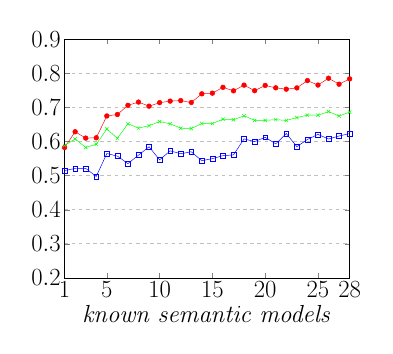
\begin{tikzpicture}[baseline,scale=0.43]
\begin{axis}[
		    xlabel={\emph{known semantic models}},
		    ylabel={},
		    xmin=1, xmax=28,
		    ymin=0.2, ymax=0.9,
		    xtick={1,5,10,15,20,25,28},
		    ytick={0.2,0.3,0.4,0.5,0.6,0.7,0.8,0.9,1},
		    legend pos=south east,
		    ymajorgrids=true,
		    grid style=dashed,
		    style = {font=\huge}
		]

		\addplot[
		    color=blue,
		    mark=square,
		    ]
		    coordinates {
		    (1,0.514832366157273)(2,0.520674170412197)(3,0.521026469009226)(4,0.497426082405143)(5,0.564688628672475)(6,0.55713561774315)(7,0.535076529852905)(8,0.560010216333054)(9,0.584508074744603)(10,0.546065110600816)(11,0.572489269396419)(12,0.564125297742057)(13,0.569829859460611)(14,0.543552852090991)(15,0.549734788036156)(16,0.558412528664919)(17,0.560598355931883)(18,0.607717979536758)(19,0.599585378842078)(20,0.612366200965436)(21,0.593021913264951)(22,0.623428063505196)(23,0.584747451140003)(24,0.605908308460775)(25,0.62089087544623)(26,0.607245006682788)(27,0.616141552483661)(28,0.623256309823247)
};
		\addplot[
		    color=red,
		    mark=*,
		    ]
		    coordinates {
		    (1,0.582318872699517)(2,0.628627876837901)(3,0.609932492636812)(4,0.610866990370165)(5,0.674948143747368)(6,0.679265687227716)(7,0.70619376828754)(8,0.715634190728361)(9,0.703653042970976)(10,0.714021677870418)(11,0.718515409501215)(12,0.72006314095146)(13,0.714534069979324)(14,0.739946209262199)(15,0.741872691279687)(16,0.759026528736177)(17,0.748648620477246)(18,0.765437399193282)(19,0.749182097087044)(20,0.764528564841459)(21,0.757553110476648)(22,0.753597067073318)(23,0.757298299109379)(24,0.778783553420146)(25,0.765628808466358)(26,0.785689475530164)(27,0.768145186235277)(28,0.783815747353212)
};
		\addplot[
		    color=green,
		    mark=x,
		    ]
		    coordinates {
		    (1,0.58839328678273)(2,0.607758082933845)(3,0.58226798181609)(4,0.591999006493134)(5,0.636658963454311)(6,0.609378189548976)(7,0.65198352100422)(8,0.639237266085298)(9,0.646381524706678)(10,0.658451931832802)(11,0.651981340743635)(12,0.639000646239548)(13,0.638100886472842)(14,0.652718769812707)(15,0.65270159785683)(16,0.665279840041019)(17,0.663658936249597)(18,0.675430261986635)(19,0.662138443878962)(20,0.662006475337153)(21,0.664124779844034)(22,0.661879115723149)(23,0.670248656767086)(24,0.677264055645277)(25,0.676979334359473)(26,0.687880411346927)(27,0.67459653454876)(28,0.68627902145454)
};
		
		\end{axis}
\end{tikzpicture}
\subcaption{Precision (museum)}\label{fig:museumprec}
\end{minipage}%
\begin{minipage}[b]{.5\linewidth}
\centering
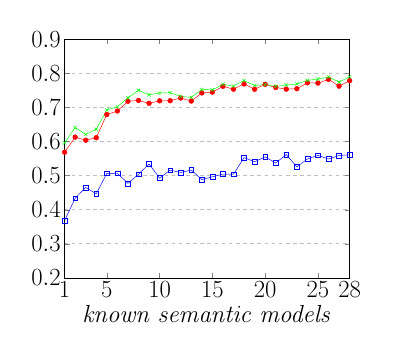
\begin{tikzpicture}[baseline,scale=0.43]
		\begin{axis}[
		    xlabel={\emph{known semantic models}},
		    %ylabel={recall},
		    xmin=1, xmax=28,
		    ymin=0.2, ymax=0.9,
		    xtick={1,5,10,15,20,25,28},
		    ytick={0.2,0.3,0.4,0.5,0.6,0.7,0.8,0.9,1},
		    ymajorgrids=true,
		    grid style=dashed,
		    		    style = {font=\huge},
		    legend style={at={(0.5,1.1)},anchor=south, legend columns=-1}
		]

		\addplot[
		    color=blue,
		    mark=square,
		    ]
		    coordinates {
		    (1,0.367995759495435)(2,0.43314958257729)(3,0.465102732953193)(4,0.446507314880989)(5,0.506469092210478)(6,0.506789578789452)(7,0.477080991784194)(8,0.503937397649502)(9,0.534229842849261)(10,0.492507267102593)(11,0.515796460946058)(12,0.509165531142068)(13,0.516097781643373)(14,0.488160651098756)(15,0.496282029692244)(16,0.504382820425249)(17,0.503923406733149)(18,0.552759367968562)(19,0.540550359776821)(20,0.554759177609889)(21,0.53688314428863)(22,0.561628603103704)(23,0.525601546354885)(24,0.548689620179471)(25,0.559372079917562)(26,0.54849327148799)(27,0.558777769863011)(28,0.561036686567106)
};
		\addplot[
		    color=red,
		    mark=*,
		    ]
		    coordinates {
		    (1,0.568526176536315)(2,0.612789529917517)(3,0.603758658205161)(4,0.611122761022995)(5,0.679226888229885)(6,0.689545922126768)(7,0.718173517817693)(8,0.72049339757837)(9,0.712025690044822)(10,0.719376710211083)(11,0.719738340274138)(12,0.727571790593847)(13,0.718652567615389)(14,0.742375410864123)(15,0.744789115461273)(16,0.761896901012414)(17,0.753562034501087)(18,0.768934123583718)(19,0.753381510225111)(20,0.767814904456983)(21,0.758472395730288)(22,0.753685690354242)(23,0.754906882661518)(24,0.772285894201019)(25,0.771337684854641)(26,0.782427299035871)(27,0.762524256400432)(28,0.778430045086962)
};
		\addplot[
		    color=green,
		    mark=x,
		    ]
		    coordinates {
		    (1,0.596084829534507)(2,0.640760186457491)(3,0.62082780704382)(4,0.636003942692136)(5,0.692664734541117)(6,0.701974230777832)(7,0.728319438123534)(8,0.750185705723487)(9,0.736888107321033)(10,0.742404159647386)(11,0.743250566844835)(12,0.732378757282814)(13,0.729581368486718)(14,0.7525692913614)(15,0.751549245497265)(16,0.767850111275969)(17,0.762600014025882)(18,0.778934826315818)(19,0.764342969952451)(20,0.767198788345341)(21,0.761867162993121)(22,0.765611676236013)(23,0.768814394670878)(24,0.779481328123055)(25,0.783142085550363)(26,0.789525770002408)(27,0.774378390471089)(28,0.790117094780008)
};
		 %\legend{karma,serene,serene-pats}

		\end{axis}
	\end{tikzpicture}
\subcaption{Recall (museum)}\label{fig:museumrec}
\end{minipage}%

\begin{minipage}[b]{.5\linewidth}
\centering
\hspace*{-15pt}
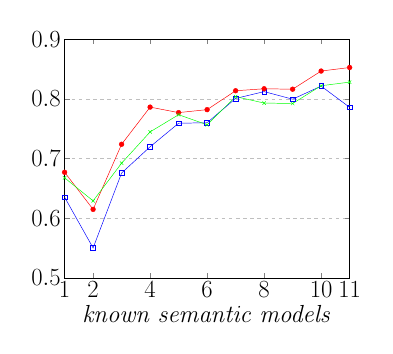
\begin{tikzpicture}[baseline,scale=0.43]
\begin{axis}[
		    xlabel={\emph{known semantic models}},
		    ylabel={},
		    xmin=1, xmax=11,
		    ymin=0.5, ymax=0.9,
		    xtick={1,2,4,6,8,10,11},
		    ytick={0.5,0.6,0.7,0.8,0.9,1},
		    legend pos=south east,
		    ymajorgrids=true,
		    grid style=dashed,
		    		    		    style = {font=\huge},
		]

		\addplot[
		    color=blue,
		    mark=square,
		    ]
		    coordinates {
		    (1,0.635191626901633)(2,0.549997502815009)(3,0.675720834727361)(4,0.719693253328935)(5,0.759169846724195)(6,0.760054331456753)(7,0.800812140122402)(8,0.812192030050689)(9,0.799552066440611)(10,0.821470975418344)(11,0.785878855002637)
		    };
		\addplot[
		    color=red,
		    mark=*,
		    ]
		    coordinates {
		    (1,0.676934852587026)(2,0.61473599870339)(3,0.723937079602602)(4,0.786238815638129)(5,0.777035817669233)(6,0.781984613615049)(7,0.81368099248534)(8,0.817013725291758)(9,0.816270530687007)(10,0.846744827831784)(11,0.852649148301322)
		    };
		\addplot[
		    color=green,
		    mark=x,
		    ]
		    coordinates {
		    (1,0.66759959719914)(2,0.629014687197419)(3,0.692208378950833)(4,0.744652988406557)(5,0.773486992410165)(6,0.756607637648352)(7,0.803820434917082)(8,0.793054493090329)(9,0.792256229657042)(10,0.822093203062231)(11,0.828181360184871)
		    };
		%\legend{karma,serene,serene-pats}

		\end{axis}
\end{tikzpicture}
\subcaption{Precision (soccer)}\label{fig:soccerprec}
\end{minipage}%
\begin{minipage}[b]{0.5\linewidth}
\centering
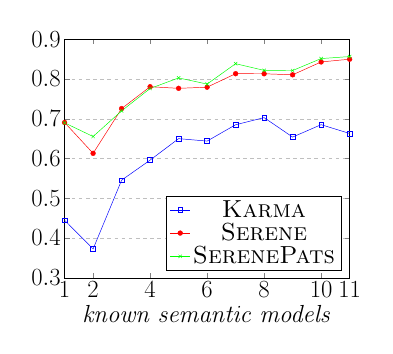
\begin{tikzpicture}[baseline,scale=0.43]
		\begin{axis}[
		    xlabel={\emph{known semantic models}},
		    %ylabel={recall},
		    xmin=1, xmax=11,
		    ymin=0.3, ymax=0.9,
		    xtick={1,2,4,6,8,10,11},
		    ytick={0.3,0.4,0.5,0.6,0.7,0.8,0.9,1},
		    ymajorgrids=true,
		    grid style=dashed, legend pos=south east,
		    		    		    style = {font=\huge}
		]

		\addplot[
		    color=blue,
		    mark=square,
		    ]
		    coordinates {
		    (1,0.444761527680188)(2,0.372447158105053)(3,0.545528381345078)(4,0.596008831526073)(5,0.6499887923799)(6,0.643884492868159)(7,0.685035675993026)(8,0.702870161195933)(9,0.654001538724769)(10,0.685153350715964)(11,0.662999993217779)
		    };
		\addplot[
		    color=red,
		    mark=*,
		    ]
		    coordinates {
		    (1,0.690636806043505)(2,0.613080486764697)(3,0.72563707600459)(4,0.780625908674911)(5,0.776616927805676)(6,0.779496772132888)(7,0.813459305700685)(8,0.813245834960899)(9,0.810586300672508)(10,0.84298404022542)(11,0.849899398175261)
		    };
		\addplot[
		    color=green,
		    mark=x,
		    ]
		    coordinates {
		    (1,0.689786194666577)(2,0.655399210040359)(3,0.719915653815835)(4,0.776231754935929)(5,0.802770096610387)(6,0.787355423564135)(7,0.838616573256072)(8,0.82175912881902)(9,0.821414409345444)(10,0.851497334083541)(11,0.85656084018153)
		    };
\legend{\karma{},\serene{},\serenepats{}}

		\end{axis}
	\end{tikzpicture}
\subcaption{Recall (soccer)}\label{fig:soccerrec}
\end{minipage}%
\caption{Performance for the museum and soccer domains. 
Average size of integration graphs for the museum domain: 88 nodes and 1129 
edges.
Average run time for the museum domain: \serene{} 0.5s, \karma{} 0.5s, \serenepats{} 1s. \label{fig:perf}}
\vspace{-3mm}
\end{figure}


% karma vs serene vs serene-pats
We evaluate our new system \serene{} and its modification \serenepats{}, which 
uses graph patterns, against the state-of-the-art system \karma{}.
All three systems have access to the same set of matches produced by our semantic labeling model.
Fig.~\ref{fig:perf} show their performance on the museum and soccer domains.
We report average precision and recall for the systems with regard to variable 
number of semantic models in the training set.
For \serene{} and \serenepats{} we report the first solutions found by
\chuffed{}. All three systems find solutions in less than a second in average.
We use default parameters for \karma{} which were shown to yield the best 
results~\cite{taheriyan2016learning}.
As we can see, \serene{} produces on average the best semantic models in terms 
of precision while \serenepats{} generates slightly better models in terms of 
recall.
If we consider results separately per each instance and not on average, there 
are few instances where \karma{} generates more precise models, however, our 
new approaches produce much better models in terms of recall in all considered 
instances. 
%%%%%%%%%%%%%%%%%%%%%%%%%%%%%%%%%%%%%%

%% sequential solution
In Fig.~\ref{fig:loo} we show how the performance of \serene{} changes 
across sequentially found solutions.
\chuffed{} successively finds better solutions in terms of Eq. \ref{EQ:obj}, 
however,
that does not translate directly into more precise semantic models.
On average, we have observed that \serene{} yields very good results already 
with the first solution found, and plateaus after the third solution.

Additionally, we investigate how the performance is influenced by introducing 
a weighting scheme on the patterns, i.e., costs of patterns are scaled by a 
factor.
In Fig.~\ref{fig:perf} we use a scaling factor 1 
for pattern costs.
When trying scaling factors 5, 10 or 20 for patterns costs from the museum 
domain we can generate semantic models which 
are almost 90\% in precision and recall.
This is a 20\% improvement in precision compared to the first solution found 
with a scaling factor of 1, and a 10\% improvement both in precision and recall 
for the first solution from \serene{}.
Contrarily to \serene{}, \serenepats{} with scaled factors produced better 
solutions in terms of precision over time.
However, the sequential solutions are not always better, and hitting the 
optimal solution may take hours.

We have also observed that \serenepats{} manages to find the ground truth on 
many instances among its sequential solutions.
This property of our approach can be used to configure various parameters for the model, e.g., scaling factors for pattern costs or match score.


% change in performance if we look at sequentially found solutions
% only leave-one-out for museum domain with 15s timeout for chuffed

\begin{figure}[!ht]\small
\centering
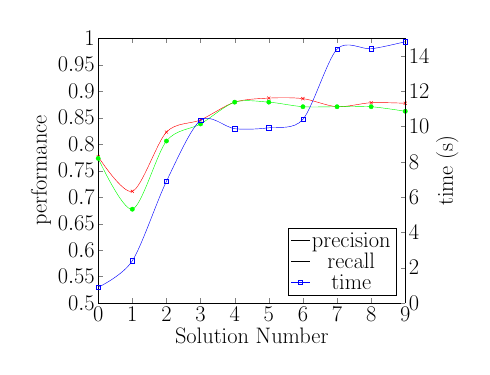
\begin{tikzpicture}[scale=0.39]
\pgfplotsset{
    scale only axis,
    xmin=0, xmax=9
}

\begin{axis}[
  axis y line*=left,
  ymin=0.5, ymax=1,
  xlabel=Solution Number,
  ylabel=performance,
  		    		    style = {font=\huge}
]
\addplot[smooth,mark=x,red]
  coordinates{
    (0,0.776507549540743)(1,0.71093042754513)(2,0.822783653218436)(3,0.845760233918129)(4,0.879310344827586)(5,0.88695652173913)(6,0.885964912280702)(7,0.870689655172414)(8,0.878260869565217)(9,0.87719298245614)

}; \label{plot_one}
\addplot[smooth,mark=*,green]
  coordinates{
    (0,0.773180507486795)(1,0.677202255831871)(2,0.805899400726987)(3,0.838122605363985)(4,0.879310344827586)(5,0.879310344827586)(6,0.870689655172414)(7,0.870689655172414)(8,0.870689655172414)(9,0.862068965517241)
}; \label{plot_two}
\end{axis}

\begin{axis}[
  axis y line*=right,
  axis x line=none,
  ymin=0, ymax=15,
  legend pos=south east,
  ylabel=time (s),
  		    		    style = {font=\huge}
]
\addlegendimage{/pgfplots/refstyle=plot_one}\addlegendentry{precision}
\addlegendimage{/pgfplots/refstyle=plot_two}\addlegendentry{recall}
\addplot[smooth,mark=square,blue]
  coordinates{
    (0,0.894338290115883)(1,2.39426428574782)(2,6.89703391393025)(3,10.3563708686829)(4,9.87668780326843)(5,9.92719115257263)(6,10.4045292949677)(7,14.3818371582031)(8,14.4026180458069)(9,14.8023208427429)
}; \addlegendentry{time}
\end{axis}
\end{tikzpicture}
\caption{Performance of \serene{} for leave-one-out strategy on the museum 
domain.}\label{fig:loo}
\vspace{-3mm}
\end{figure}

%\npr{Maybe some words on how optimal solution found by chuffed relates to the ground truth?}

\section{Related Work \label{SEC:pw}}

Relational data sources are still one of the most popular ways to store enterprise or Web data, however, the issue with relational schema is the lack of a well-defined semantic description.
A common ontology provides a way of representing the meaning of a relational 
schema and can facilitate the integration of heterogeneous data sources within 
a domain.
Indicating semantic correspondences manually might be appropriate if only few data sources need to be integrated, however, it becomes tedious with the growing number of heterogeneous schemata.
Hence, automatic or semi-automatic approaches for relational-to-ontology schema mapping are being actively developed.


The majority of approaches to solve the \relonto{} mapping problem are based on 
heuristic rules and alignment of constraints specified within relational 
schemata and ontologies.
A very comprehensive overview and comparison of existing mapping generation 
tools based on this approach is given by~\citeasnoun{Pinkel:rodi}
and~\citeasnoun{Spanos:semweb}.
As examples, there are BootOX~\cite{Jimenez:Bootox}, MIRROR~\cite{Luciano:Mirror} and  ontop~\cite{Fagin:Clio}.
Crudely speaking, these tools first apply a default direct mapping specified by the W3C.
Further, the default ontology is enriched by using explicit and implicit schema constraints.
Finally, ontology alignment techniques are applied to match the default ontology to the target ontology.
The main advantage of these systems is the ability to run in a fully automatic setting.
Our approach is complementary to the approaches from this group and at its current stage is semi-automatic.
However, constraint programming offers a convenient framework to incorporate integrity constraints specified either within relational or ontological schema as additional constraints to govern the search for the solution.
This opens an interesting direction for further research.

A major issue with fully automatic systems is that constraints may be 
inconsistent or absent completely, e.g., data from Web services or tables on 
the Web.
To overcome this issue, we can apply ML techniques.
\citeasnoun{Limaye:Annotating} design a system to annotate web tables with 
entities for cell values, semantic labels for attributes and relationships for 
binary combinations of attributes.
As in our approach, they decompose the process of mapping into two main stages: semantic labeling and finding relationships between matched semantic labels.
\citeasnoun{Limaye:Annotating} enrich their data sources by using YAGO.
\citeasnoun{Mulwad:Semantic} extend this approach by leveraging information 
from Wikitology Knowledge Base (KB).
\citeasnoun{Venetis:Recovering} develop a scalable approach to recover the 
semantics of Web tables by incorporating data from the isA database KB.
\citeasnoun{Ritze:matching}, on the other hand, use DBPedia as their KB.
%extract additional data from knowledge bases to assign a semantic label to an attribute.
Hence, these approaches are limited to domains well represented in those knowledge bases.
Also, they are not able to find the relation between attributes in the table if there is no direct connection between the attributes.
Our approach, on the other hand, allows a model to be trained on any data and can infer complex semantic paths which might exist between attributes.
However, it might be further bootstrapped by leveraging external knowledge bases.
This is especially beneficial at the start when the system does not have sufficient training data.

As mentioned above, the approaches for mapping Web tables also perform semantic labeling.
They design various similarity metrics for attribute names and values.
However, they disregard the attributes which are not matched to the ontology 
(the so-called \emph{unknown} set of attributes) which are especially abundant 
on the Web~\cite{Ritze:matching,Pham:semantic}.
It is clear that we cannot directly speak about similarity for unmatched attributes, since they are rather dissimilar from known semantic types.
That is why we have developed a new approach for semantic labeling which can efficiently handle the \emph{unknown} class.
We demonstrate its efficiency by comparing against the state-of-the-art approach DSL~\cite{Pham:semantic}.

We build upon the work of \citeasnoun{taheriyan2016learning} and use their 
ideas for the construction of the alignment graph.
The only difference is that we introduce the \emph{unknown} and \emph{root} class nodes and as many \emph{unknown} data nodes as there are attributes in the modeled data source.
These nodes serve to capture the unmatched attributes from the source.
Though we have modified \karma{} to treat these additional nodes as well, our 
approach outperforms \karma{} since we have additional constraints for these 
nodes and use an exact algorithm to solve the STP.
\citeasnoun{taheriyan2016learning} treat the matching and STP parts of \relonto{} independently and use heuristic algorithms for both.
We, on the other hand, use exact algorithms for both parts and address them within a unified CP model.

In their follow up work, \citeasnoun{Taheriyan:Leveraging} suggest using graph 
patterns to boost the performance of their system.
To this end, they had to revise their algorithm by introducing additional heuristics.
However, in our case we only had to add pattern variables and to modify the 
objective function in the \minizinc{} model.
No changes to the solver were required.
This makes our system very convenient and opens directions for validating various additional constraints.
\ignore{Though our approach beats the state-of-the-art in the conducted 
experiments, it 
is worth noting that the scalability of our approach is under question.
The main argument why exact solution for STP is feasible in our setting is that 
we map data sources to a domain-specific ontology which is expected to be 
limited in its size.}

\section{Conclusion}
In this paper we have introduced a new approach, \serene{} (and its extension 
that uses frequent graph patterns, \serenepats{}) to solve the problem of 
relational-to-ontology schema mapping.
Our experiments demonstrate that 
\serene{} generates on average more consistent semantic models in terms of 
precision and recall compared to the state-of-the-art approach \karma{}.
\serenepats{} produces, on average, better semantic models in terms of 
recall, and its precision can be enhanced by adding a scaling factor for 
pattern costs.

Furthermore, our approach is extremely flexible and easy to extend with 
arbitrary side constraints thanks to the use of CP rather than a specific 
heuristic algorithm.
\ignore{
However, the solutions discovered by \serenepats{} later tend to be 
much better both in precision and recall.
The disadvantage is though that it comes at a cost of run time.
In the end, which approach to use for the \relonto{} problem comes down to 
trade-offs between precision, recall and time.
}

\ignore{
%%%%%%%%future directions%%%%%%%%%%%%%
% cold start problem and LOD
One of the key limitations of our approach is the availability of training data 
in the domain, which is often referred to as cold start problem.
We consider leveraging the data from the Linked Open Cloud (LOD) which, on one 
hand, leads to improved performance in the light of insufficient data and, on 
the other hand, helps in publishing consistent Linked 
Data~\cite{Taheriyan:Leveraging}. 
As we have shown, the frequent graph pattern mining procedure 
DIMSpan~\cite{petermann2017dimspan} which we use in our work is a highly 
scalable approach compared to the technique based on SPARQL queries 
from~\cite{Taheriyan:Leveraging}.

%incorporate schema and ontology constraints
Incorporating schema and ontology constraints may also help with the cold start 
problem.
Furthermore, it can provide means to improve disambiguation of properties.
For example, it is hard for our system to differentiate between startDate and 
endDate of the class Event.
Having a constraint that startDate is before endDate might improve the mapping 
in such situations.

%complex matches
Another interesting direction for further research is to recognize complex 
matches.
Our semantic labeling model in \serene{} as well as many others in the 
literature~\cite{Pham:semantic,Ritze:matching} can learn only one-to-one 
matches between attributes and properties in the ontology.
\cite{Pinkel:rodi} show that such systems as BootOX can also handle efficiently 
only one-to-one matches while their performance degrades considerably for $1:n$ 
and $n:1$ matches.
\karma{} \cite{taheriyan2016learning} offers its users to manually specify 
transformations through Python scripts.
\cite{Dhamankar:imap} offer a way to learn such transformations from the 
historic data.
This is one of the features which we want to incorporate into \serene{}.
}
\bibliographystyle{aaai}
\bibliography{main}


\newpage
\section*{Appendices}
\renewcommand{\thesubsection}{\Alph{subsection}}

\subsection{Features for Semantic Labeling\label{Ann:SemLab}}

Below are the description of features used by \serene{} semantic model.
Note that features are extracted from the name and values of each attribute in the data source.
Thus, all the data from a single column is reduced to some feature
vector of the concatenation of values computed by the extractors below.
We refer to a single value from the column as an entry. For example, in the table below, John is an entry of the column Person.

\begin{table}[!ht]\small
  \centering
  \caption{Example table.}
  	\begin{tabular}{ccc} 
  		\hline
		Person & Age & Gender \\
  		\hline
	    John & 20 & M\\
    	Jane & 30 & F\\
  		\hline
		\end{tabular} 
%\vspace*{-3mm}
\end{table}


\begin{table}[h]
	\centering
	\caption{Feature extractors that produce a scalar value}
	\begin{tabular}{p{3cm}p{4.5cm}}
	Feature name & Description \\ \hline
	num-unique-vals & A simple count of unique entries of a column\\
	\rowcolor{Gray}
	prop-unique-vals & The proportion of unique entries of a column. \\
	\rowcolor{Gray}
	prop-missing-vals & The proportion of all missing/empty entries from all entries in a column.\\
	ratio-alpha-chars & The average of the proportion of alphabetic characters from each entry.\\
	\rowcolor{Gray}
	prop-numerical-chars & The average of the proportion of numeric characters from each entry.\\
	prop-whitespace-chars    & The average of the proportion of whitespace characters from each entry.\\
	\rowcolor{Gray}
	prop-entries-with-at-sign& The proportion of entries with an '@' sign. \\
	prop-entries-with-hyphen & The proportion of entries with a '-'. \\
	\rowcolor{Gray}
	prop-range-format        & The proportion of entries which follow some \\ numerical range format &  ([0-9]+)-([0-9]+) \\
	\rowcolor{Gray}
	is-discrete              & A binary indicator if the column entries are discrete. \\
	entropy-for-discrete-values & The entropy of the entries of a column.\\
	\rowcolor{Gray}	
	shannon-entropy          & Shannon's entropy for the vocabulary specified in the description of the feature 'char-dist-features'\\
	\end{tabular}
\end{table}



\begin{table}[t]
	\centering
	\caption{Feature extractors that produce a vector value. Some of these are computed together to reduce computation time.
	Others are values that are computed for all classes.}
	
	\begin{tabular}{p{2.5cm}p{5cm}}
	Feature name & Description \\ \hline
inferred-data-type      & Produces a vector which contains the inferred data type.  
Only a single element is non-zero in the vector (i.e. 1-of-K format).  
The set of inferred types are in float, integer, long, boolean, date, time, datetime, string. \\
	\rowcolor{Gray}
char-dist-features      & Produces a vector for character distribution of column values;
considered characters are printable characters
%                        0123456789abcdefghijklmnopqrstuvwxyz
%                        ABCDEFGHIJKLMNOPQRSTUVWXYZ!"
%                        #$%&\'()*+,-./:;<=>?@[\\]^_`{|}~ \t\n\r\x0b\x0c
\\
stats-of-text-length    & Computes the mean, median, mode, min, max of string lengths from a columns entries.\\
	\rowcolor{Gray}
stats-of-numerical-type & Computes the mean, median, mode, min, max of entries from a column of numerical type.\\

prop-instances-per-class-in-knearestneighbours         & This finds the k columns from the training set with most similar names.
It then produces a vector of class proportions from these k neighbours.
Parameters:
"num-neighbours": The number of neighbours to find (k).\\
	\rowcolor{Gray}
mean-character-cosine-similarity-from-class-examples   & For some test instance t, this computes the character distribution 
from this instance's entries.  It then produces a vector of the average
cosine similarity of t with training instances of each class.\\
min-editdistance-from-class-examples                   & For some test instance t, this produces a vector of the minimum column name
edit distance between t and all training instances of each class.
Parameters:
"cache-size": Size of cache for storing edit distances of words 
"max-comparisons-per-class": Max number of training instances to compare
against for each class.\\

	\rowcolor{Gray}
min-wordnet-jcn-distance-from-class-examples            & For some test instance t, this produces a vector of the minimum column name
JCN WS4J distance between t and all training instances of each class.
Parameters:
"cache-size": Size of cache for storing wordnet distances of words 
"max-comparisons-per-class": Max number of training instances to compare
against for each class.\\

min-wordnet-lin-distance-from-class-examples            & For some test instance t, this produces a vector of the minimum column name
LIN WS4J distance between t and all training instances of each class.
Parameters:
"cache-size": Size of cache for storing wordnet distances of words 
"max-comparisons-per-class": Max number of training instances to compare
against for each class.\\

\end{tabular}
\end{table}






\clearpage\newpage
\subsection{\minizinc{} Model \label{Ann:MZ}}
\renewcommand{\lstlistingname}{Model}
\begin{minipage}{\textwidth}
%\begin{figure}[!h]
	\begin{lstlisting}[caption={\minizinc{} model (part 1 of 2)},captionpos=b]
%%%%%%%%%%%%%%%%%%%%%%%%%%%%%%%%%%%%%%%%%%%%%%%%%%%%%%%%%%%%%%
%%                                                          %%
%% MiniZinc model to solve the Steiner Tree Problem arising %%
%% in the Rel2Onto problem.                                 %%
%%                                                          %%
%%%%%%%%%%%%%%%%%%%%%%%%%%%%%%%%%%%%%%%%%%%%%%%%%%%%%%%%%%%%%%

include "globals.mzn";

%%%%%%% Steiner Tree Problem
int: nbV;                               % Nb of nodes in alignment graph
int: nbE;                               % Nb of edges in alignment graph
set of int: nodes = 1..nbV;    
set of int: edges = 1..nbE;
set of int: cnodes;                     % Class nodes in alignment graph
set of int: dnodes;                     % Data nodes in alignment graph
set of int: anodes;                     % Attribute nodes in alignment graph (normally none)
array [nodes] of var bool: vs;          % Is a node of the alignment graph in the solution?
array [edges] of var bool: es;          % Is an edge of the alignment graph in the solution?
array [nodes,edges] of bool: adjacent;  % adjacent[n,e] <=> node n is an endnode of edge e
array [edges] of nodes: heads;          % endpoint 1 of each edge (the graph is undirected)
array [edges] of nodes: tails;          % endpoint 2 of each edge
array[1..2,edges] of int: endpairs = array2d(1..2,edges,tails++heads);
array [edges] of int: ws;               % Weights of edges in alignment graph
var 0..sum(ws): w;                      % Weight of the solution corresponding to the alignment part
constraint steiner_tree(vs,es,adjacent,endpairs,w,ws);  % Steiner Tree constraint
constraint forall (d in dnodes) 
                   (vs[d] <-> sum(e in edges where adjacent[d,e])(es[e]) == 1);% Only 1 edges per data node 

%%%%%%% Matching Problem
int: nbA;                                           % Nb of attribute nodes
set of int: atts = 1..nbA;                 
array [atts] of set of dnodes: attribute_domains;   % Data nodes to which each attribute can attach (usually all) 
constraint forall(att in anodes) (vs[att] == true); % Attribute nodes (normally none) are in the graph.
array [atts] of var dnodes: match;                  % Match between Attributes and Data nodes
array[atts,dnodes] of int: match_costs;             % Weight of match edges
constraint forall (a in atts) (match[a] in (attribute_domains[a]));   % Must match someone in the domain
constraint forall (a in atts) (vs[match[a]]);       % The data node matched must be in the subgraph of the alignment
constraint alldifferent(match);                     % Exact match
var 0..sum(a in atts)(sum(n in dnodes)(match_costs[a,n])): wm;  % Total cost from matching part :
constraint wm = sum(a in atts) (match_costs[a,match[a]]);

	\end{lstlisting}
%	\caption{\minizinc{} model (1/2).}
%\end{figure}
\end{minipage}
\clearpage
\newpage
\begin{minipage}{\textwidth}
%\begin{figure*}[t]
	\begin{lstlisting}[caption={\minizinc{} model (part 2 of 2)},captionpos=b]
%%%%%%% Unknown nodes
int: nb_unknown_nodes;                 % Number of unknown data nodes
set of int: unknowns = 1..nb_unknown_nodes;
array [int] of int: all_unk_nodes;     % List of all unknown nodes (first two elements are class nodes, by convention)
int: node_root = all_unk_nodes[1];     % Root node if unknown class node is used.
int: node_unk = all_unk_nodes[2];      % Unknown class node
constraint if nb_unknown_nodes > 0 then
    vs[node_unk] <-> vs[node_root]     % If class node "Unknown" is used, class node "Root" is used as well
 /\ vs[node_root] <-> sum(e in edges where adjacent[node_root,e])(es[e]) in {1,2}
else true %Ignore constraint
endif;


%%%%%%% Patterns
int: nb_patterns;                     % Number of patterns
set of int: PATTS = 1..nb_patterns;
array[PATTS] of int: patterns_w;      % Support of patterns
array[PATTS] of set of int: patterns; % The actual patterns
array[PATTS] of var bool: c_p;        % Is pattern chosen
constraint forall (p in PATTS) ((sum (e in patterns[p])   % All edges of a pattern are used <-> pattern is used
							                  	(es[e]) == card(patterns[p])) <-> c_p[p]);
var 0..sum(patterns_w): wp;           % Total prize collected from patterns : 
constraint if nb_patterns = 0 then wp = 0 else wp = sum(p in PATTS) (c_p[p] * patterns_w[p]) endif;


%%%%%%% Final objective function 
var int: obj = w + wm - wp;           % Total cost of semantic model - prize collected from patterns


%%%%%%% Search startegy
array[atts,dnodes] of int: match_costs_sorted;  % Match of attributes, sorted by cost.
ann: cheap_matches = int_search([ match[a] == match_costs_sorted[a,i] |a in atts, i in dnodes], 
                                input_order,indomain_max,complete);

array[edges] of int: sorted_edges = arg_sort(ws);
ann: cheap_edges = int_search([es[sorted_edges[nbE + 1 - e]] | e in edges],input_order,indomain_min,complete);

ann: cheap_edges_fill_pattern;        % Custom search strategy for patterns
ann: custom(ann, array[int] of int, array[int] of var bool);
array[int] of ann: cefp = 
if nb_patterns == 0 then [] 
else [custom(cheap_edges_fill_pattern,[nbE]++[nb_patterns]++ws++[ card(patterns[p]) | p in PATTS]++patterns_w++array1d([ e | p in PATTS, e in patterns[p]]),es)] endif;

% The solver will use these strategies in order:
% 1) First try using the cheapest matches matches, until a match is found
% 2) If there are patterns, use a specific search called "cheap_edges_fill_pattern". (Implemented in Chuffed only)
%    It will start adding edges in increasing order of cost, while trying to fill patterns that are "worth" filling.
%    E.g. We already set es[x] = true for x in {e1,e2,e3}; if adding ws[e5] = 4 and ws[e7] = 6, but
%    {e1,e2,e3,e7} form a pattern p of patterns_w[p] = 3, then ws[e7] - patterns_w[p] <  ws[e5], so e7 is selected first
%    If there are no patterns, this strategy is ignored.
% 3) Try to eliminate edges by decreasing cost: it will eliminate the more expensive edges first, until
%    the strictly necesary cheap edges are added by the propagators. This is used only when there are no 
%    patterns, otherwise (2) already selects the edges.

solve ::seq_search([cheap_matches]++cefp++[cheap_edges]) 
minimize obj;
	\end{lstlisting}
	%\caption{\minizinc{} model (2/2).}
%\end{figure*}
\end{minipage}

















\ignore{
%% sequentially found solutions and different weights for patterns
\begin{figure*}[h]\small
\pgfplotsset{
    small,
    %legend style={legend pos=north east}
    legend style={
        at={(0.01,0.01)},
        anchor=south west,
    },
   }%
\begin{minipage}[b]{.34\linewidth}
\centering
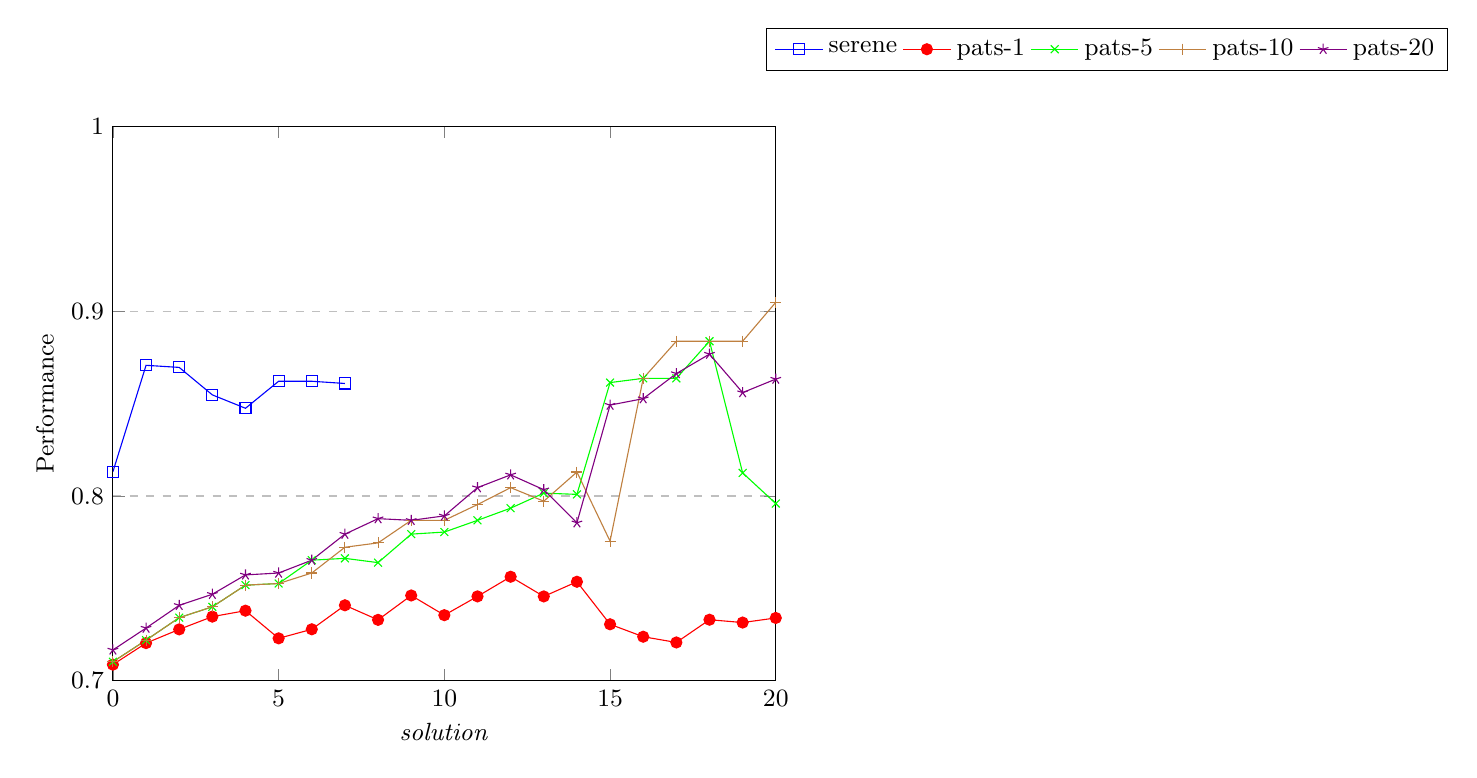
\begin{tikzpicture}[baseline]
\begin{axis}[
		    xlabel={\emph{solution}},
		    ylabel={Performance},
		    xmin=0, xmax=20,
		    ymin=0.7, ymax=1,
		    xtick={0,5,10,15,20},
		    ytick={0.7,0.8,0.9,1},
		    legend pos=south east,
		    ymajorgrids=true,
		    grid style=dashed,
		    legend style={at={(1.5,1.1)},anchor=south, legend columns=-1}
		]

		\addplot[
		    color=blue,
		    mark=square,
		    ]
		    coordinates {
		    (0,0.813133718212162)(1,0.870689655172414)(2,0.869565217391304)(3,0.854700854700855)(4,0.847457627118644)(5,0.862068965517241)(6,0.862068965517241)(7,0.860869565217391)
		    };
		\addplot[
		    color=red,
		    mark=*,
		    ]
		    coordinates {
		    (0,0.708791208791209)(1,0.720429778415431)(2,0.727852084972463)(3,0.734756097560976)(4,0.737969058591178)(5,0.723003960808839)(6,0.727905921593153)(7,0.740887177292826)(8,0.733003960808839)(9,0.746193299741805)(10,0.73554304773817)(11,0.74569890495285)(12,0.756325773784054)(13,0.745676961413577)(14,0.753615746683783)(15,0.7306060898002)(16,0.723882805154582)(17,0.720774744968293)(18,0.733079110976868)(19,0.731544715447155)(20,0.734034752112227)

		    };
		\addplot[
		    color=green,
		    mark=x,
		    ]
		    coordinates {
		    (0,0.71031746031746)(1,0.722023912003826)(2,0.734193548387097)(3,0.740054370716392)(4,0.751788722391459)(5,0.752652119278914)(6,0.765286464150101)(7,0.766275317871063)(8,0.763956676916058)(9,0.779373522458629)(10,0.780497706328908)(11,0.786846912678115)(12,0.793409626193882)(13,0.801554001554001)(14,0.800878033205619)(15,0.861352657004831)(16,0.863636363636364)(17,0.863636363636364)(18,0.883720930232558)(19,0.8125)(20,0.795918367346939)
		    };
		\addplot[
		    color=brown,
		    mark=+,
		    ]
		    coordinates {
		    (0,0.71031746031746)(1,0.722023912003826)(2,0.734193548387097)(3,0.740054370716392)(4,0.751788722391459)(5,0.752652119278914)(6,0.758342019705656)(7,0.772281323877069)(8,0.774638933587619)(9,0.786846912678115)(10,0.786846912678115)(11,0.795363644516187)(12,0.804524886877828)(13,0.797201562617384)(14,0.812955643390426)(15,0.775568181818182)(16,0.863636363636364)(17,0.883720930232558)(18,0.883720930232558)(19,0.883720930232558)(20,0.904761904761905)
};
		 \addplot[
		    color=violet,
		    mark=star,
		    ]
		    coordinates {
		    (0,0.716727716727717)(1,0.728559859716244)(2,0.740860215053763)(3,0.746857091804827)(4,0.757315933275812)(5,0.758342019705656)(6,0.765286464150101)(7,0.779373522458629)(8,0.787744083140503)(9,0.786846912678115)(10,0.789244481875285)(11,0.804524886877828)(12,0.811442006269593)(13,0.803401771336554)(14,0.785524847694936)(15,0.849173553719008)(16,0.852651515151516)(17,0.866230213015439)(18,0.876750700280112)(19,0.85593220338983)(20,0.863247863247863)
};
		\legend{serene,pats-1,pats-5,pats-10,pats-20}

		\end{axis}
\end{tikzpicture}
\subcaption{precision}\label{fig:solprec}
\end{minipage}%
%
\begin{minipage}[b]{.33\linewidth}
\centering
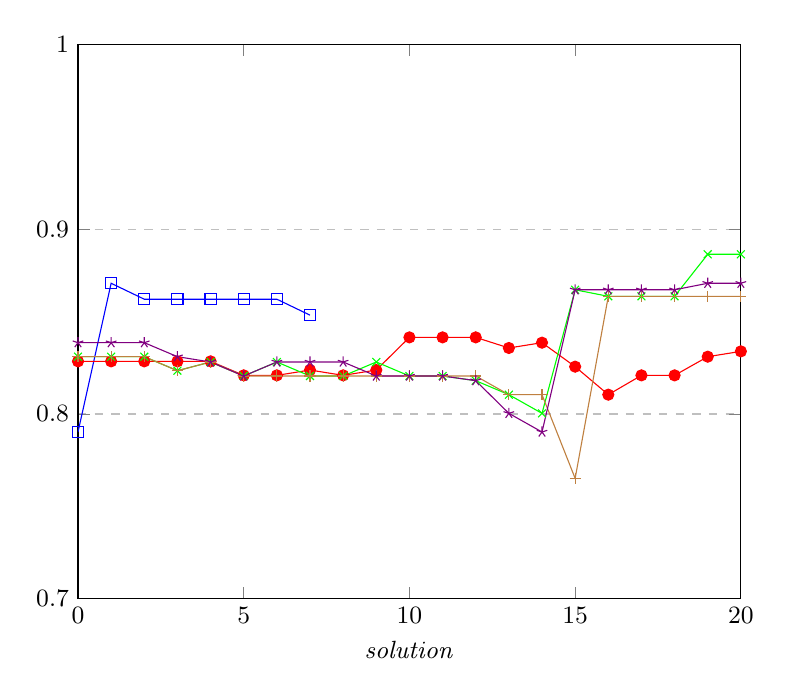
\begin{tikzpicture}[baseline]
		\begin{axis}[
		    xlabel={\emph{solution}},
		    %ylabel={recall},
		    xmin=0, xmax=20,
		    ymin=0.7, ymax=1,
		    xtick={0,5,10,15,20},
		    ytick={0.7,0.8,0.9,1},
		    ymajorgrids=true,
		    grid style=dashed,
		    %legend style={at={(0.5,1.1)},anchor=south, legend columns=-1}
		]

		\addplot[
		    color=blue,
		    mark=square,
		    ]
		    coordinates {
		    (0,0.790229885057471)(1,0.870689655172414)(2,0.862068965517241)(3,0.862068965517241)(4,0.862068965517241)(5,0.862068965517241)(6,0.862068965517241)(7,0.853448275862069)
		    };
		\addplot[
		    color=red,
		    mark=*,
		    ]
		    coordinates {
		    (0,0.828456983629397)(1,0.828456983629397)(2,0.828456983629397)(3,0.828456983629397)(4,0.828456983629397)(5,0.82088122605364)(6,0.82088122605364)(7,0.823754789272031)(8,0.82088122605364)(9,0.823754789272031)(10,0.841431556948798)(11,0.841431556948798)(12,0.841431556948798)(13,0.835684430512017)(14,0.838557993730407)(15,0.825583420411007)(16,0.810431905259492)(17,0.82088122605364)(18,0.82088122605364)(19,0.83098223615465)(20,0.833855799373041)
};
		\addplot[
		    color=green,
		    mark=x,
		    ]
		    coordinates {
		    (0,0.83098223615465)(1,0.83098223615465)(2,0.83098223615465)(3,0.823406478578892)(4,0.828108672936259)(5,0.820532915360502)(6,0.828108672936259)(7,0.820532915360502)(8,0.820532915360502)(9,0.828108672936259)(10,0.820532915360502)(11,0.820532915360502)(12,0.818007662835249)(13,0.810431905259492)(14,0.800330895158482)(15,0.867163009404389)(16,0.863636363636364)(17,0.863636363636364)(18,0.863636363636364)(19,0.886363636363636)(20,0.886363636363636)
};
		 \addplot[
		    color=brown,
		    mark=+,
		    ]
		    coordinates {
		    (0,0.83098223615465)(1,0.83098223615465)(2,0.83098223615465)(3,0.823406478578892)(4,0.828108672936259)(5,0.820532915360502)(6,0.820532915360502)(7,0.820532915360502)(8,0.820532915360502)(9,0.820532915360502)(10,0.820532915360502)(11,0.820532915360502)(12,0.820532915360502)(13,0.810431905259492)(14,0.810431905259492)(15,0.765151515151516)(16,0.863636363636364)(17,0.863636363636364)(18,0.863636363636364)(19,0.863636363636364)(20,0.863636363636364)
};
		 \addplot[
		    color=violet,
		    mark=star,
		    ]
		    coordinates {
		    (0,0.838557993730407)(1,0.838557993730407)(2,0.838557993730407)(3,0.83098223615465)(4,0.828108672936259)(5,0.820532915360502)(6,0.828108672936259)(7,0.828108672936259)(8,0.828108672936259)(9,0.820532915360502)(10,0.820532915360502)(11,0.820532915360502)(12,0.818007662835249)(13,0.800330895158482)(14,0.790229885057471)(15,0.867163009404389)(16,0.867163009404389)(17,0.867163009404389)(18,0.867163009404389)(19,0.870689655172414)(20,0.870689655172414)
};	
	%\legend{serene,pats-1,pats-5,pats-10,pats-20}
		\end{axis}
	\end{tikzpicture}
\subcaption{recall}\label{fig:solrec}
\end{minipage}%
%
\begin{minipage}[b]{.33\linewidth}
\centering
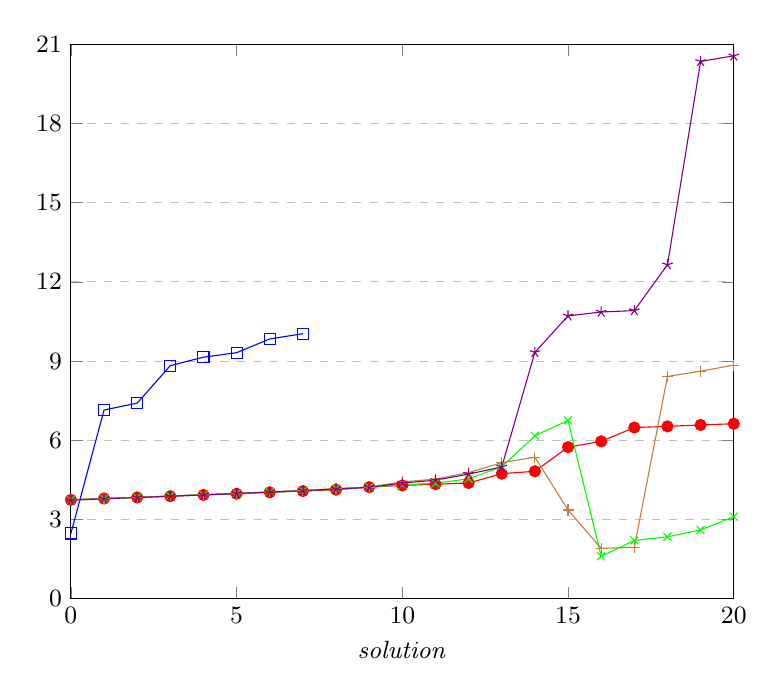
\begin{tikzpicture}[baseline]
\begin{axis}[
		    xlabel={\emph{solution}},
		    %ylabel={time(s)},
		    xmin=0, xmax=20,
		    ymin=0.0, ymax=21,
		    xtick={0,5,10,15,20},
		    ytick={0.0,3.0,6.0,9.0,12,15.0,18,21.0},
		    ymajorgrids=true,
		    grid style=dashed,
		    %legend pos=outer north east,
		    %legend style={at={(0.5,-0.1)},anchor=north, legend columns=-1}
		]

		\addplot[
		    color=blue,
		    mark=square,
		    ]
		    coordinates {
		    (0,2.47666666666667)(1,7.15)(2,7.41)(3,8.83)(4,9.15)(5,9.32)(6,9.84)(7,10.04)
};
		\addplot[
		    color=red,
		    mark=*,
		    ]
		    coordinates {
		    (0,3.75)(1,3.8)(2,3.84)(3,3.88666666666667)(4,3.93333333333333)(5,3.98)(6,4.03333333333333)(7,4.08)(8,4.13333333333333)(9,4.23)(10,4.29333333333333)(11,4.34)(12,4.38666666666667)(13,4.74)(14,4.83)(15,5.74333333333333)(16,5.96333333333333)(17,6.48666666666667)(18,6.53)(19,6.58333333333333)(20,6.63)
};
		\addplot[
		    color=green,
		    mark=x,
		    ]
		    coordinates {
		    (0,3.74)(1,3.79)(2,3.83666666666667)(3,3.88666666666667)(4,3.93666666666667)(5,3.98666666666667)(6,4.03666666666667)(7,4.09333333333333)(8,4.17333333333333)(9,4.23)(10,4.31666666666667)(11,4.38)(12,4.54333333333333)(13,5)(14,6.17666666666667)(15,6.755)(16,1.61)(17,2.21)(18,2.35)(19,2.61)(20,3.11)
};
		\addplot[
		    color=brown,
		    mark=+,
		    ]
		    coordinates {
		    (0,3.75)(1,3.8)(2,3.84666666666667)(3,3.89666666666667)(4,3.95)(5,3.99666666666667)(6,4.05)(7,4.10333333333333)(8,4.16666666666667)(9,4.23333333333333)(10,4.43)(11,4.53333333333333)(12,4.78)(13,5.15333333333333)(14,5.36333333333333)(15,3.365)(16,1.91)(17,1.95)(18,8.42)(19,8.62)(20,8.85)
};
		 \addplot[
		    color=violet,
		    mark=star,
		    ]
		    coordinates {
		    (0,3.73666666666667)(1,3.78666666666667)(2,3.83666666666667)(3,3.88333333333333)(4,3.93666666666667)(5,3.98666666666667)(6,4.04333333333333)(7,4.09666666666667)(8,4.16)(9,4.22)(10,4.38333333333333)(11,4.49)(12,4.72333333333333)(13,4.99333333333333)(14,9.33333333333333)(15,10.715)(16,10.86)(17,10.915)(18,12.65)(19,20.35)(20,20.56)
};	
	%\legend{serene,pats-1,pats-5,pats-10,pats-20}
		\end{axis}
\end{tikzpicture}
\subcaption{time (s)}\label{fig:soltime}
\end{minipage}%
\caption{Average precision, recall and time on the museum domain for leave-one-out strategy and different weighting scheme for patterns in serene.}\label{fig:perfsol}
\end{figure*}

}

\ignore{

\begin{table}[ht]\small
  \centering
  \caption{Run times (s) for all instances on the museum domain}\label{tab:time}
		\begin{tabular}{cccc}
		\hline
		System & Mean & Min & Max\\
		\hline
		karma & 0.48 & 0.19 & 2.3  \\
		serene & 0.53 & 0.01 & 8 \\
		serene-pats & 0.97 & 0.01 & 20.3 \\
		\hline
		\end{tabular} 
\end{table}
\begin{table}[ht]\small
  \centering
  \caption{Sizes of integration graphs on the museum domain}\label{tab:size}
		\begin{tabular}{cccc}
		\hline
		 & Mean & Min & Max\\
		\hline
		number of nodes & 87.8 & 29 & 168  \\
		number of edges & 1129.4 & 88 & 5629 \\
		\hline
		\end{tabular} 
\end{table}
}

\end{document}
